%!TEX root = ../thesis.tex
%*******************************************************************************
%****************************** Second Chapter *********************************
%*******************************************************************************

\chapter{Medical Background}
\label{chapter1}

\ifpdf
    \graphicspath{{Chapter2/Figs/Raster/}{Chapter2/Figs/PDF/}{Chapter2/Figs/}}
\else
    \graphicspath{{Chapter2/Figs/Vector/}{Chapter2/Figs/}}
\fi

Measuring blood flow provides valuable information to the clinical community about the healthiness of either organs or limbs. Being capable of estimate instant blood flow of one of the limbs provide information about how blood flow is ultimately reaching these extremities that could avoid ischemia (\textit{isch} in Greek means to stop or block and \textit{emia} that means blood flow) or amputation caused by a non-proper perfusion to the extremity. In fact, if there were indicators about either venous or arterial occlusion could provide a clue about how to proceed with the proper treatment.

\mynote{This introduction needs to be improved. More about what I'm going to describe should be added}

The following chapter describes the importance of blood flow, the problems and complications derived from a poorly perfused limb could cause. During the continuation of the reading, some of the current technologies will be explained and what methods are used to estimate blood flow currently.  

\section{Circulatory system} %section 2.1
\label{section literature 1}
The human body has a closed circulatory system, where the blood is enclosed within the blood vessels and is transported to and from the heart that works as a pump. The main function of the circulatory system is to carry oxygen and nutrients to all the cells in the body but also collecting their metabolic process byproduct. Blood flows through vessels that form a complex, elastic tubular network that reaches each cell of the body. The arteries carry oxygenated blood, and the veins return deoxygenated blood. 

Blood moves from the arterial to venous circulation within the capillaries. Plasma passes through capillaries that are only a thick cell in diameter. Then, the blood pressure increases by forcing fluid out of the capillary walls, which is known as interstitial fluid. In the end, some of this fluid returns to the capillaries, and some go to the lymphatic vessels. The different components of the circulatory system will be described in more detail in the following sections. Especially arms anatomy as is the part of the body that will be tested by the device designed. 

\subsection{The blood}
Blood is the main carrier of nutrients that runs through humans and vertebrate animals. It also takes a major part in the body's defence combating infections. In short, it is in charge of transporting oxygen and collecting carbon dioxide from all the tissues that constitute the body.  Blood requires of different paths to circulate in the human body; the circulatory system is used to carry oxygenated and deoxygenated blood, also known as arterial and venous blood respectively. Indeed, the body uses arteries to transport oxygenated blood coming out from the heart and uses veins to return deoxygenated blood to the heart.

\mynote{Add a description of which veins are involved in the periphery and how works in the arm. Arm Anathomy}
%********************************** %Section 2.1.1.1  **************************************  
\subsubsection{The blood plasma}
\label{section literature 1.1}
It is important to describe the plasma as one of the main electrical conductors in the human body. The plasma is the suspending medium where the blood cells described by table \ ref {table: cell} travel around the body. Indeed the extracellular fluids originate from the plasma's fluid.

The solutes inside the plasma play important roles at a cellular level. Within it amino acids, glucose and vitamins are dissolved to be used by the cellular metabolic process. Also, there are present hormones that regulate the blood cell activity and their chemical residuals such as nitrogen ($N$) and $CO_2$.

The plasma is mainly composed of salt and water. In fact, it is quite similar to seawater but with a lower concentration of ions. Some of them present in significant numbers are sodium ($Na$), chloride ($Cl^-$)and bicarbonate ($HCO_3^-$) ions. However, there are also traces of calcium, magnesium, copper, potassium and zinc.

Proteins are also present in the plasma that are produced by the liver. The most common are albumin, but there are alpha and beta globulins that convey lipids and steroids hormones, and \textit{fibrinogen} used during the clotting process.

%********************************** %Section 2.1.1  **************************************  
\subsubsection{Blood cells}
\label{section literature 1.2}
There are well known and identifiable components in blood. Approximately, half of its volume is constituted of plasma which properties were described previously and the other half of red blood cells (erythrocytes), white blood cells (leukocytes or monocytes) and platelets (thrombocytes). In short, red blood cells function is to transport oxygen; the white blood cells are in charge of the immunological response, and platelets of the clotting process.

However, these cells also perform other specialised tasks. Their properties and characteristics are described more in detail in table \ref{table:cell}, it also includes cells quantity per microliter (\si{\micro\litre}) of human blood. It must be noted that there are diverse specialised subtypes of white cells and platelets but not further details of this cells will be covered in this work.

\begin{table}
\caption{Blood cell classification}
\label{table:cell}
\centering
\begin{tabular}{p{2.5cm} p{1.5cm} p{3.5cm} p{6.5cm}}
\toprule
\textbf{Cell Type }& \textbf{Quantity} & \textbf{Geometry} & \textbf{Characteristic} \\
\midrule
Red Blood Cells (RBCs ) \newline or erythrocytes & \numrange{5e6}{6e6} & Shape: Disk \newline Diameter: 6-\SI{8}{\micro\meter} \newline Thickness: \SI{2}{\micro\meter} & 
\begin{tabular}[t]{@{\textbullet~}p{6.5cm}@{}} 
    Principal medium to deliver oxygen \\
    Lack of nucleus \\
    Cytoplasm rich in negatively charged Iron–containing Hb \\
    Contains Ions of Sodium ($Na^+$) and Potassium ($K^+$) \\
    Typical bilayer lipid membrane (Lipid composition defies physical properties such as membrane permeability and fluidity) 
\end{tabular} \\
\midrule

White Blood Cells (WBC) \newline or Monocytes & \numrange{4e3}{11e3} & Shape: Irregular \newline Diameter: 10–\SI{20}{\micro\meter} \newline Monocytes: 14–17 & 
\begin{tabular}[t]{@{\textbullet~}p{6.5cm}@{}} 
    Composed five different type of specialised cells to target different illnesses\\
    Make part of the immune system \\
    High count of these cells are indicators of disease 
\end{tabular} \\
\midrule

Platelets & \numrange{150e3}{400e3} & Shape: Irregular \newline Diameter: 2–\SI{3}{\micro\meter}  &  
\begin{tabular}[t]{@{\textbullet~}p{6.5cm}@{}}
    Lack of nucleus  \\
    Responsible for procoauglant activity \\
    If count to low excessive blood may occur. Too high blood cloth might form (thrombosis)
\end{tabular} \\ 

\bottomrule
\end{tabular}
\end{table}

\subsection{Blood vessels}
The blood leaves the heart through the arteries that reach all the organs of the body. This network of vessels branches to a microscopic size, at this point they are called arterioles. Then, blood enters the capillaries, which are tiny thin-walled tubes that reach the size of a cell. Venules collect the blood that comes out of the capillaries and then moves to the main veins, which carry it back to the heart.

Arteries, arterioles, veins and venules are composed of the same cellular structure (see figures \ref{fig:arteries composion} and \ref{fig:veins composion}). The innermost part of these vessels is an epithelial coating known as the endothelium. A thin layer of elastic fibres, a smooth muscle and connective tissue, lies around the endothelium. Capillaries are much thinner compared to these vessels. Indeed, capillaries are made only of endothelium cells which allow the exchange of fluids between the blood and the surrounding tissue (see figure \ref{fig:capillaries composion}). This interchange of molecules and ions between both occurs by diffusion, by filtration at the capillary walls, and by transport trough endothelial cells. Hence, it is here where the exchange of gases and metabolites occurs between blood and the body cells \cite{johnson2001biology}.

\begin{figure*}[!htbp]
	\centering
	\begin{subfigure}[t]{0.33\textwidth}
		\centering
		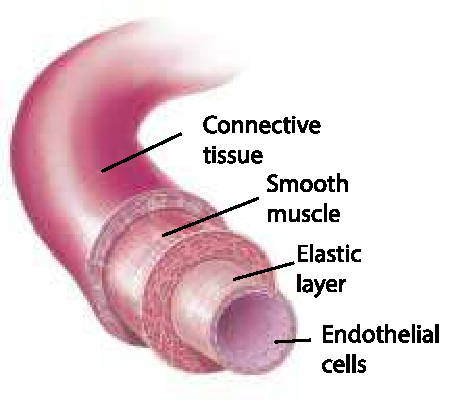
\includegraphics[width=5cm]{figure1a}
		\caption{Layers of the arteries}
		\label{fig:arteries composion}
	\end{subfigure}%
	~ 
	\begin{subfigure}[t]{0.33\textwidth}
		\centering
		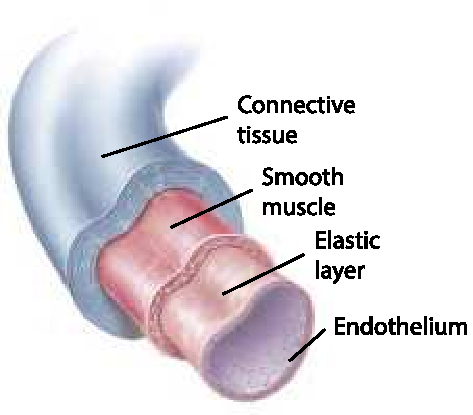
\includegraphics[width=5cm]{figure1c}
		\caption{Layers of the venous}
		\label{fig:veins composition}
	\end{subfigure}
	~ 
	\begin{subfigure}[t]{0.33\textwidth}
		\centering
		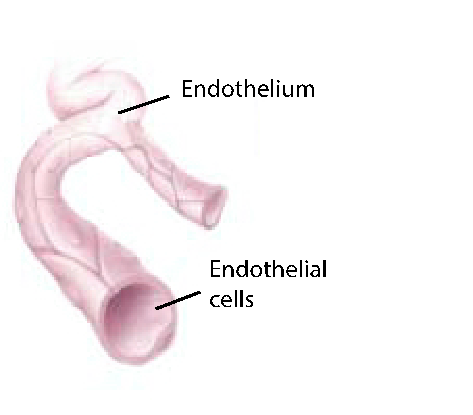
\includegraphics[width=5cm, trim={0 0 2cm 0},clip]{figure1b}
		\caption{Layers of the capillaries}
		\label{fig:capillaries composition}
	\end{subfigure}
	\caption[Layers of the blood vessels]{The arteries and veins have the same kind of layers. However, the smooth muscle is thicker in arteries than veins. The capillaries have a thin wall and are composed only by endothelium. Figure adapted from \cite{johnson2001biology}.}
	\label{fig:vessels composition}
\end{figure*}

\subsubsection{Arteries and arterioles}
The arteries slightly differ from the arterioles in their composition. The main arteries contain additional elastic fibres within them, enabling greater compliance while receiving blood coming out the heart. On the other hand, smaller arteries and arterioles contain thicker smooth muscle layer in their tunica media allow them to resist bursting.  

There is a direct relation between the diameter of the vessel and the frictional resistance to blood flow. The resistance to blood flow is inversely proportional to the radius of the vessel. Halving the diameter of a blood vessel increases 16 times its frictional resistance. Hence, the greatest resistance to blood flow in this branch of the circulatory system occurs in the small arteries and arterioles. Moreover, when the smooth muscle layer of the arterioles contracts, it produces vasoconstriction, which increases resistance and decreases blood flow. On the other hand, when this muscle relaxes vasodilation occurs, dropping resistance and increasing blood flow. Local chemical factors, the sympathetic system or hormones can control both muscle activities. Furthermore, blood flow towards some organs can also be regulated by precapillary sphincters. These rings of smooth muscle can shut down capillary beds totally. For instance, in cold weather, these precapillary sphincters may close to contribute to the vasoconstriction limiting heat loss.  

\subsubsection{Capillaries}
As it was described before, the capillaries are considerable smaller than the rest of the blood vessels. On average, every one of them is about \SI{1}{\milli\meter} long and \SI{8}{\micro\meter} diameter, just big enough to allow a single RBC (\SIrange{6}{8}{\micro\meter}) pass through. The capillary tree is so dense and extensive that every cell in the human body is within \SI{100}{\micro\meter} of reach.  Due to the enormous amount of them and their intricate network,  they have the greatest cross-section area of any other kind of blood vessel. Therefore, the blood decreases its velocity allowing more time to exchange metabolites with the surrounding extracellular fluid. As soon as the blood has left the capillary, all the exchange of $O_2$, nutrients, $CO_2$ and waste products have taken place. 

It must be noted, that the heart must produce enough pressure to overcome the resistance of the blood passing the arterial tree into the capillaries. However, blood loses most of its pressure when moving through the capillary network but also passes to a low-pressure system when entering to the veins. 

\subsubsection{Venules and veins}
Venules collect the blood that leaves the capillaries and then is deposited in the larger veins that lead the blood back to the heart. Because the pressure in the venous return is one-tenth of the arteries, venules and veins contain a thinner layer of smooth muscle. This pressure gradient also helps the blood to pass through the narrow passages of the capillaries. Most of the blood volume is contained within the veins, which also have the ability to expand to increase the body's blood capacity if needed. In order to help the blood return from the extremities, the surrounding skeletal muscle contracts by compressing the veins pushing the blood back to the heart. Also, the veins contain valves that only allow blood to flow in one direction. However, sometimes these valves may fail to lead to a vascular problem such as varicose veins. 

\begin{figure}[!htpb]
	\centering
	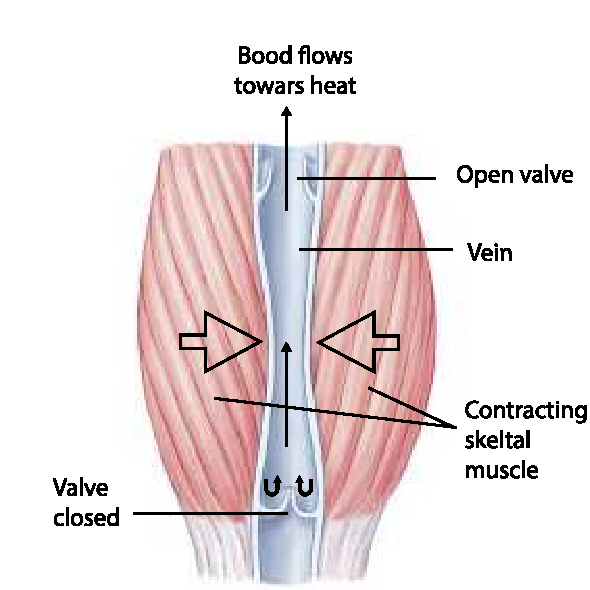
\includegraphics[width=0.5\textwidth,keepaspectratio]{figure2}    
	\caption[Venous return through skeletal muscle]{The vein only flows in on direction helped by valves along the vessel. Skeletal muscle contraction aids the return of blood to the heart. Figure adapted from \cite{johnson2001biology}. }
	\label{fig:venous return}
\end{figure}

\section{Cardiac cycle}
It is important to understand how the heart operates because changes of volume are synchronous to the heart beating. As part of the circulatory cycle, the heart has to overcome the pressure of pushing RBC's through the capillaries. Hence, the heart has to go work as a dual pump, pushing out arterial and collecting venous blood. The cardiac cycle is a periodic task that starts at the beginning of one heart beat until the start of the following one. The cycle is divided into ventricular contraction known as systole and ventricular relaxation called diastole. 

Each cardiac cycle is subdivided into phases where the heart experiences intense pressure change at constant volume or a volume change with a minor alteration in pressure. During the systolic cycle the heart experiences (1) isovolumetric contraction followed by (2) blood ejection. On the other hand, diastole cycle follows the next steps (1) isovolumetric relaxation, (2) early diastolic filling,(3) slow ventricular filling (diastasis) and (4) atrial filling \cite{fukuta2008cardiac}. The heart rate is inversely proportional to the cardiac cycle and changes according to the body's needs. An average heart rate is about 75 beats per minute, where a single beat last around \SI{0.8}{\second}.

At resting, the duration of the systolic cycle takes about 1/3 of the total heart cycle and the diastolic cycle 2/3. At high heart rate during exercise, this rate proportion changes, the duration of diastole takes much less time than the systole one. The following sections will describe the changes on the heart, as well as pressures, electrical activity and heart sounds all along each cycle.

\subsection{Systole}
\subsubsection{Isovolumetric contraction}
As his name suggests iso (greek equal) volumic (volume) contraction, in this stage the heart keeps the same blood volume while the ventricles contract.
\mynote{I have to double check the etymology of this word}
\begin{figure}[!htpb]
	\begin{subfigure}[t]{0.48\textwidth}
		\centering
		\raisebox{1.25cm}{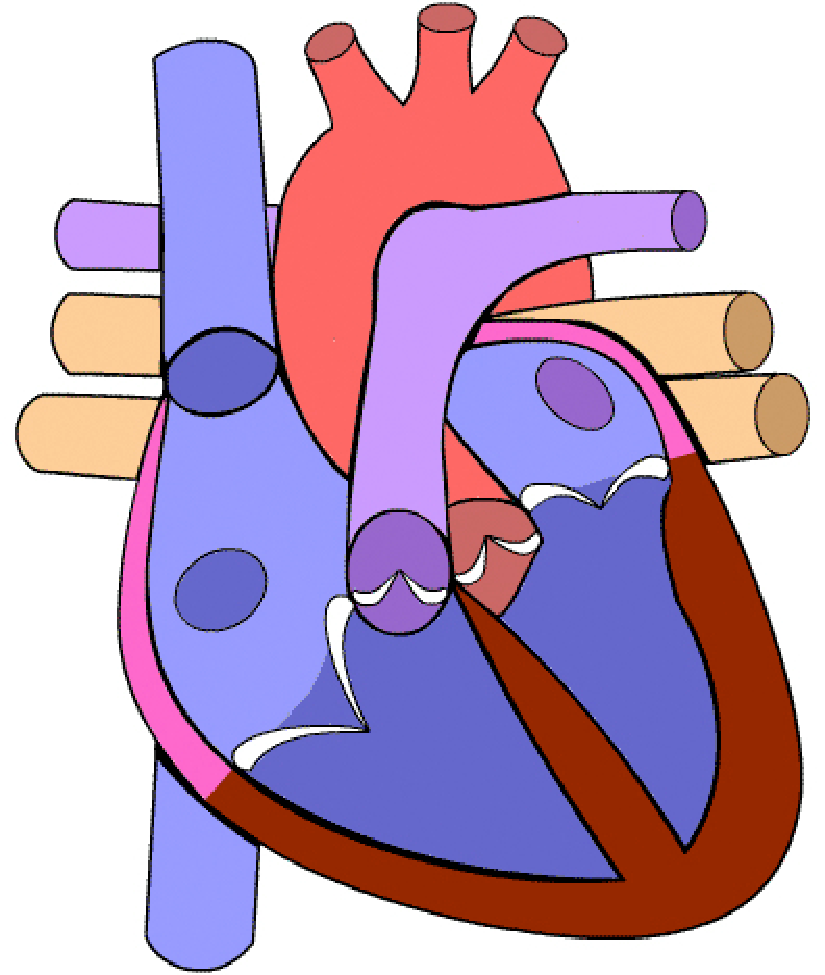
\includegraphics[height=6cm,keepaspectratio]{figure_3}}    
		\caption{Cross section of the heart during isovolumetric contraction. The contracted area is represented by the red colour.}
		\label{fig:heart isovolumic}
	\end{subfigure}
	~
	\begin{subfigure}[t]{0.48\textwidth}
		\centering
		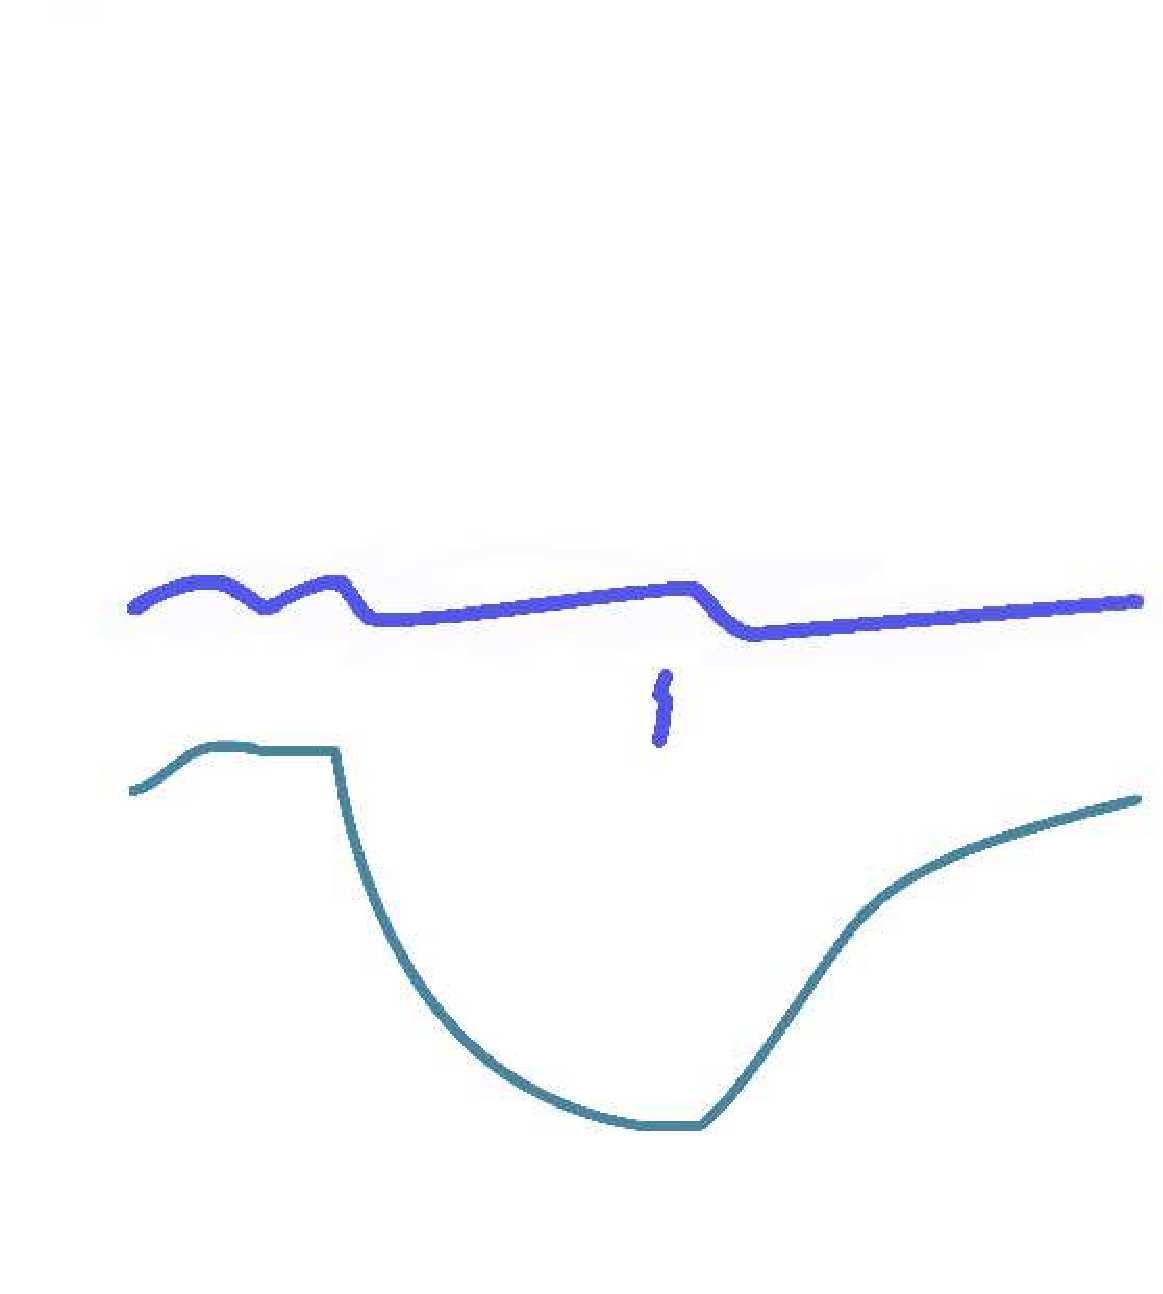
\includegraphics[width=\textwidth,keepaspectratio]{figure_4}    
		\caption{Pressures and volume changes during isovolumetric contraction in the highlighted area. In red the pressure of the left ventricle, in black the aortic pressure, dark blue the pressure of the right atrium and light blue the ventricular volume.}
		\label{fig:pressure isovolumic}
	\end{subfigure}
	\caption{Isovolumetric contraction in the heart and changes of pressure and volumes}
\end{figure}

Figure \ref{fig:pressure isovolumic} shows the variation of pressure in the left ventricle, the right atrium, the aortic pressure and the ventricular volume. As the valves are shut, and the ventricles are contracted, and blood can not leave the heart, thus the ventricular pressure increases but there is no change in the blood's volume. In the end, the total volume inside the ventricles is equivalent to the end-diastolic volume (about \SI{130}{\milli\litre}. In the atria, due to the differential of pressure between chambers the atrioventricular bulges backwards. Therefore, this valve change causes a small variation of pressure in the right atrium. It is depicted as the point c in the figure same figure. The pressure in the systemic and pulmonary arteries drops at a constant rate. 

\mynote{I need to reference this to the website.}

\mynote{If I have time, I should get this data and create my own plot.}

The electrocardiogram waveform is shown in figure \ref{fig:ECG isovolumic} displays the electrical activity of the heart during this section of the cycle. In short, the depolarization of the heart starts from the atrioventricular node spreading through the bundle of His and Purkinje fibres to the septum and the walls of both ventricles. This event causes the QRS complex shown in the same figure. At the same time, the atrial repolarisation causes the atrial T wave which is not visible in the ECG because QRS complex covers it.

\begin{figure}[!htpb]
	\centering
	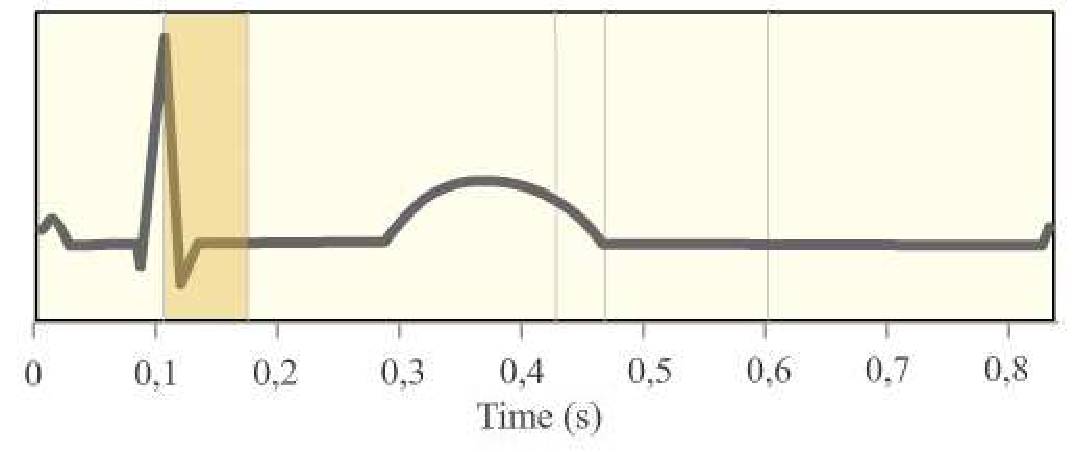
\includegraphics[width=0.5\textwidth,keepaspectratio]{figure_5}    
	\caption[Isovolumic contraction - ECG]{ECG during isovolumic contraction.}
	\label{fig:ECG isovolumic}
\end{figure}

\mynote{Maybe this can be explained by another form simpler. Check if I need the echocardiography part unless I match this part with the paper about echo.}

\subsubsection{Ejection}
During this cycle, the mechanics of the heart experiences the following changes. The gradient of pressure is greater in the left ventricle compared to the one in the aorta. Also, the increasing pressure of the right ventricle exceeds the one in the pulmonary artery. Hence, the semilunar valves open. Due to the ventricular contraction, the blood is ejected from both ventricles to the aorta and pulmonary arteries. Moreover, the atrioventricular valves are closed.

\begin{figure}[!htpb]
\begin{subfigure}[t]{0.48\textwidth}
	\centering
	\raisebox{1.25cm}{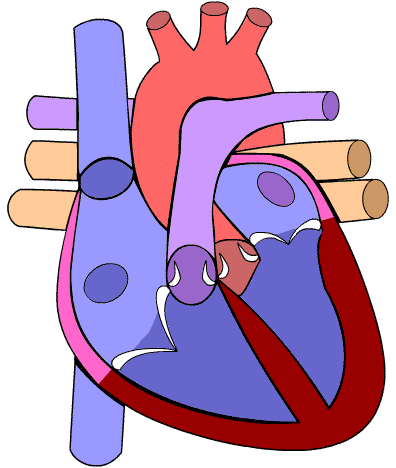
\includegraphics[height=6cm,keepaspectratio]{figure_6}}
	\caption{Cross section of the heart during the ejection cycle. The contracted area is represented by the red colour. The semilunar valves are open.}
	\label{fig:heart ejection}
\end{subfigure}
~
\begin{subfigure}[t]{0.48\textwidth}
	\centering
	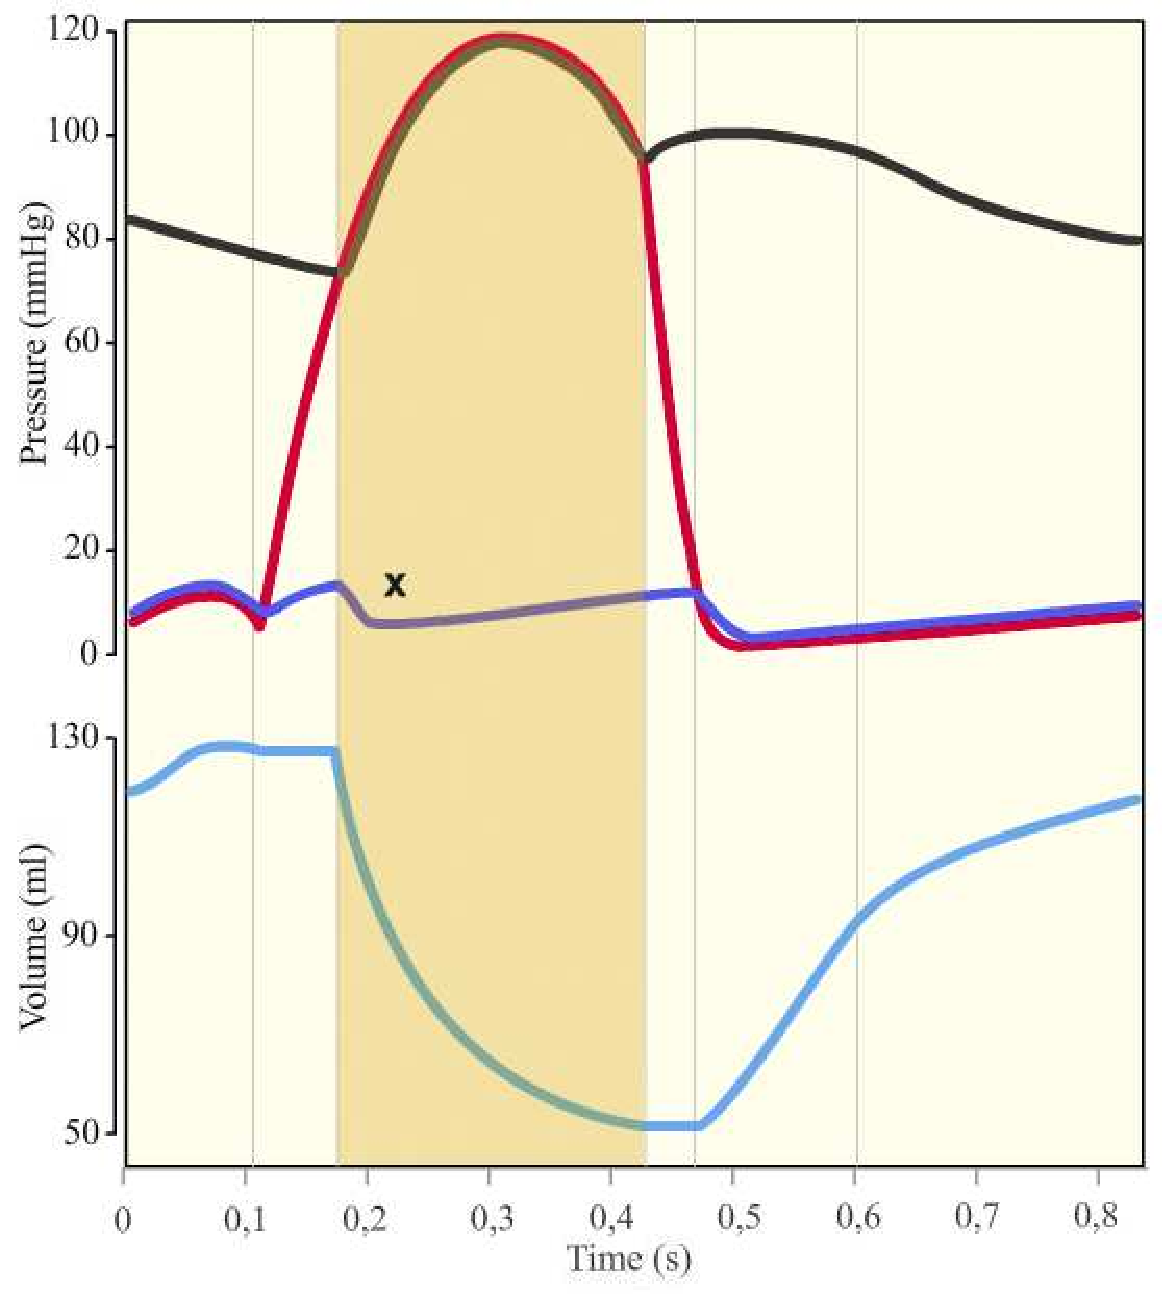
\includegraphics[width=\textwidth,keepaspectratio]{figure_7}
	\caption{Cross section of the heart during the ejection cycle. The contracted area is represented by the red colour. The semilunar valves are open.}
	\label{fig:pressure ejection}
\end{subfigure}
	\caption[Heart's ejection]{Mechanical changes, variation of pressure and volume during ejection cycle.}
\end{figure}

More in detail, this cycle divides into a rapid and slow ejection. Regarding pressure, the increasing ventricular pressure during the contraction creates the sudden purge of blood toward the arteries. Then, the blood volume within the ventricles and arteries begins to drop. Due to the pressure difference between these two, the blood is ejected slowly. During this cycle, normally the maximum pressure of left ventricular reaches about \SI{120}{\mmHg}, which is known as systolic pressure and \SI{25}{\mmHg} in the right ventricle. These pressures are also transferred to the aorta and pulmonary arteries respectively which also start to drop after reaching these peaks. Regarding blood volume, under normal conditions while resting only \SI{70}{\milli\litre} of blood is ejected, this is known as the stroke or systolic volume. The rest \SI{60}{\milli\litre} remains in the heart until the end of the cycle which is known as end-systolic volume. The relation between stroke volume and the end-diastolic volume is known as ejection fraction being \SI{60}{\percent} the normal physiological range. The atria also contract all along this cycle. The pressure in the atria and main vein vessels decreases because they being elongated by the shortening of the ventricles. Hence, there is a drop in the atria's pressure. 

\begin{figure}[!htpb]
	\centering
	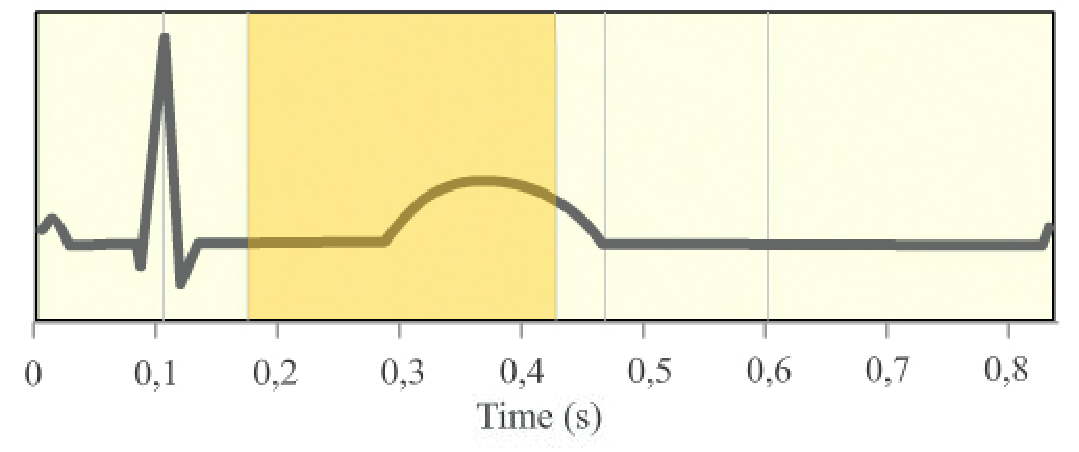
\includegraphics[width=0.5\textwidth,keepaspectratio]{figure_8}
	\caption[Heart's ejection]{Cross section of the heart during the ejection cycle. The contracted area is represented by the red colour. The semilunar valves are open.}
	\label{fig:ECG ejection}
\end{figure}

From the electrical point of view, at the beginning of this cycle, the ventricles are completely depolarised which is equivalent to the ST segment of the electrocardiogram. Due to ventricular repolarisation, the T wave can be seen in the second part of this stage. 

\subsection{Diastole}
\subsubsection{Isovolumetric relaxation}
In the heart's mechanics, once the heart completes its systole the ventricles relax, and the pressure starts to drop rapidly. Then, due blood inertia for a short period the blood flows out of the ventricles. The elevated pressures in the aorta and pulmonary arteries pushes back a little bit of blood towards the ventricle, but this also closes the semilunar valves. Also, the atrioventricular valves are closed because the pressure in the atria is lower than the one in the ventricle.

\begin{figure}[!htpb]
	\begin{subfigure}[t]{0.48\textwidth}
		\centering
		\raisebox{1.25cm}{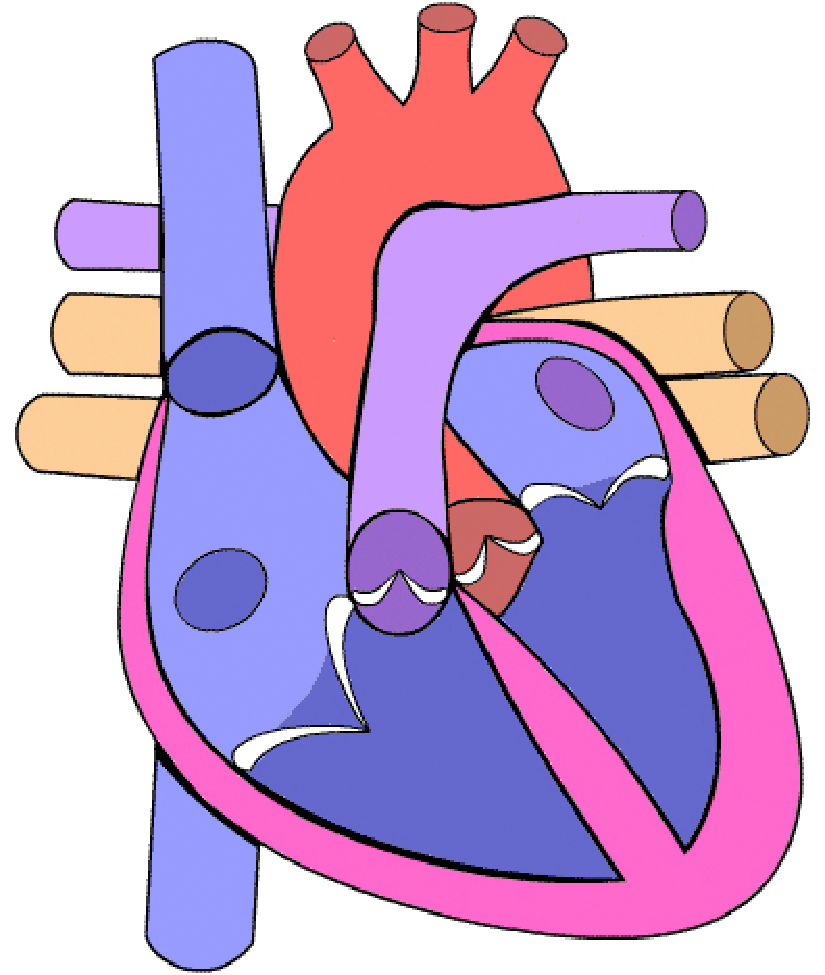
\includegraphics[height=6cm,keepaspectratio]{figure_9}}
		\caption{Cross section of the heart during the isovolumetric relaxation cycle. Semilunar and atrioventricular valves are closed in this stage.}
		\label{fig:heart isovolumetric relaxation}
	\end{subfigure}
	~
	\begin{subfigure}[t]{0.48\textwidth}
		\centering
		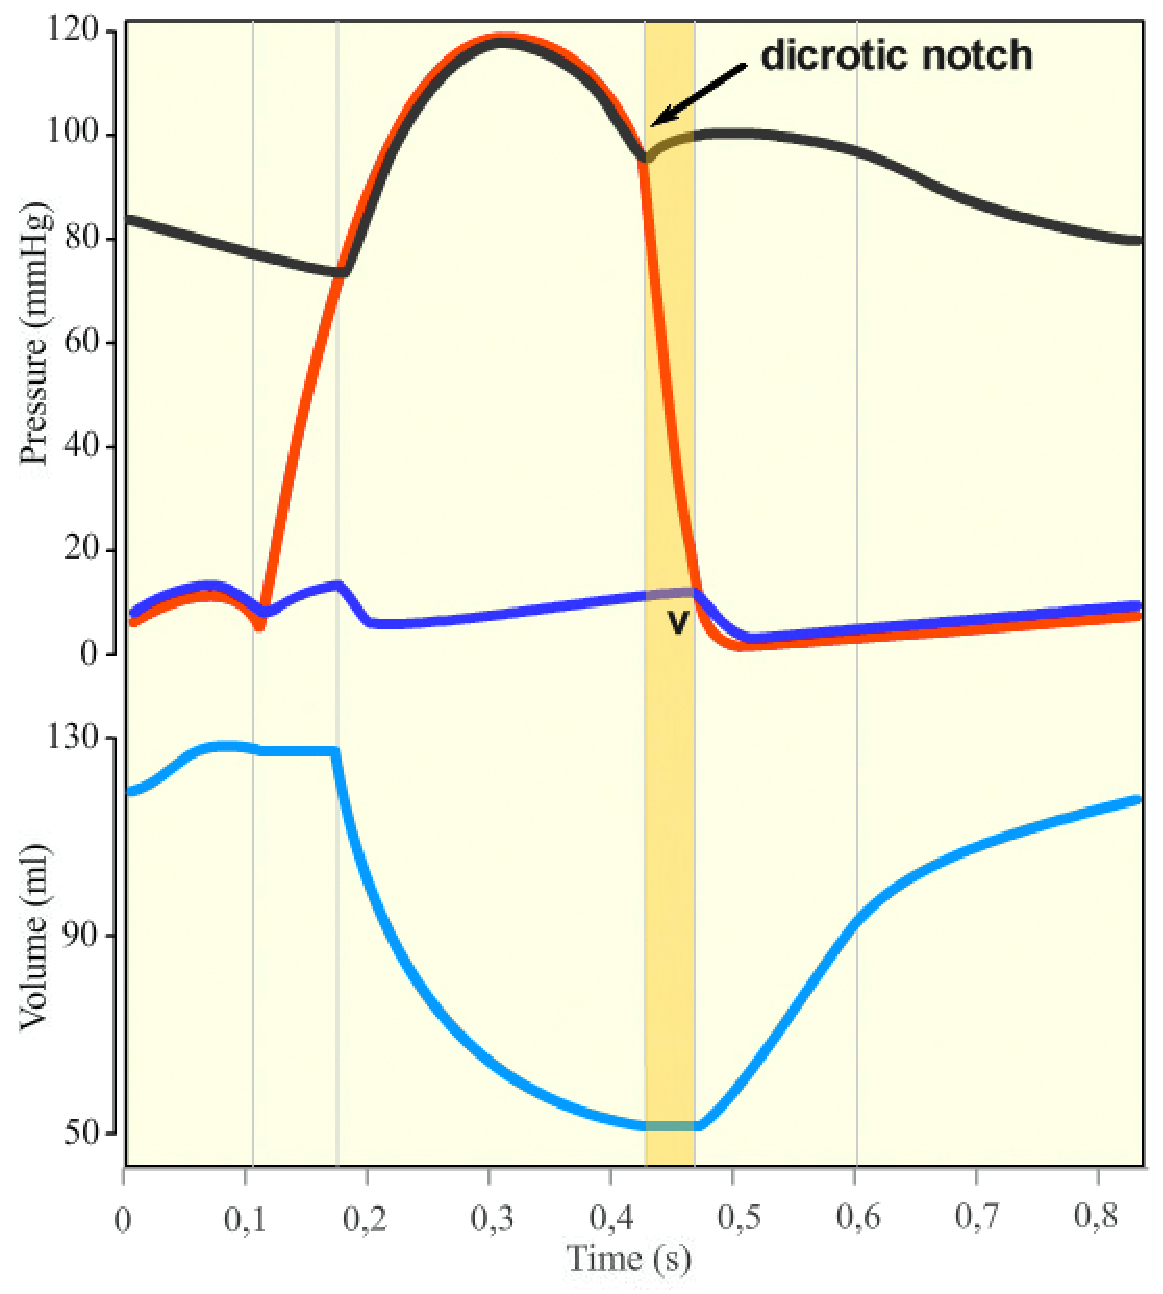
\includegraphics[width=\textwidth,keepaspectratio]{figure_10}
		\caption{During isovolumetric relaxation the ventricles are relaxed but the volume within the ventricles (light blue) remain the end-systolic volume (\SI{60}{\milli\litre}). The blood flowing backwards is shown by an small increase in the arterial pressure (black line). The pressure in the ventricle reduces nearly to zero (red line).}
		\label{fig:pressure isovolumteric realxation}
	\end{subfigure}
	\caption[Isovolumetric relaxation]{Heart's mechanical changes, pressure and volume change during isovolumetric relaxation}
\end{figure}

The changes of pressures and volumes in the different chambers occurs as follows. The ventricles relax rapidly decreasing their pressure without altering the blood volume. Hence the name isovolumetric relaxation. Indeed, the blood remaining within the ventricle is still the end-systolic volume (\SI{60}{\milli\litre}. This relaxation period also causes a great drop in ventricular pressure until getting close to zero in both ventricles at the end this cycle. The atria are filled with blood from the veins while the atrioventricular valves remain closed. This action increases the pressure in atria (v wave in the plot). In the arteries, the decrease of their pressure is interrupted by the dicrotic notch which is a temporary increase in pressure that also creates a blood backflow which also closes the semilunar valves. 

During this period, the ventricle is completely repolarised completing the T wave in the ECG as shown in the figure.

\begin{figure}[!htpb]
	\centering
	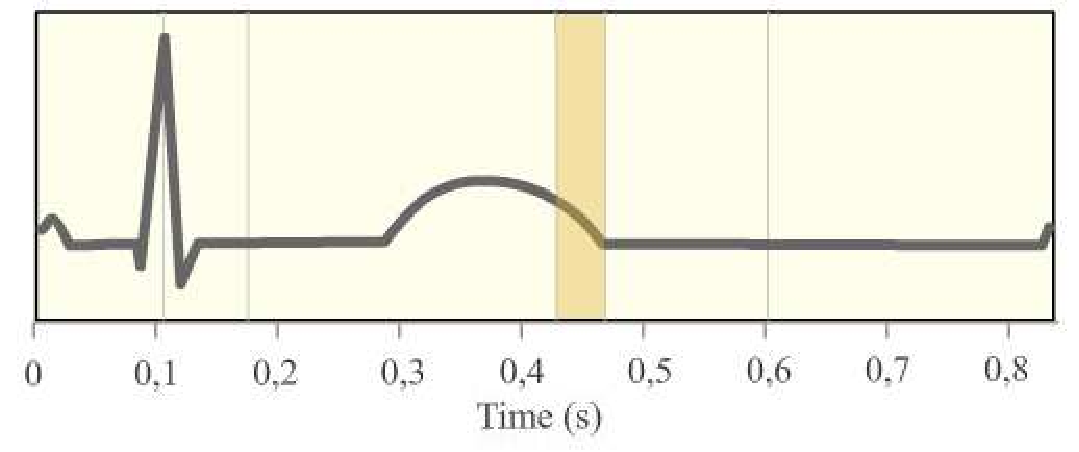
\includegraphics[width=0.5\textwidth,keepaspectratio]{figure_11} 
	\caption[Isovolumetric relaxation in ECG]{During isovolumetric relaxation the ventricle is completely repolarised completing the T wave.}
	\label{fig:ECG isovolumetric relaxation}
\end{figure}

\mynote{Change the captions of this figures}

\subsubsection{Rapid ventricular filling}
During this cycle, the ventricular pressure reaches a point where is lower than the atrial one. Therefore, the atrioventricular valves open allowing the blood accumulated in the atria passing quickly to the ventricles. Most of the ventricular filling occurs during this stage. Also, the blood volume within the ventricle increases but its pressure changes insignificantly due to the muscle relaxation. In the atria, there is a decrease in pressure (seen as venous pulse y wave) caused by the blood rushing out from the atria to the ventricles. 
\begin{figure}[!htpb]
	\begin{subfigure}[t]{0.48\textwidth}
		\centering
		\raisebox{1.25cm}{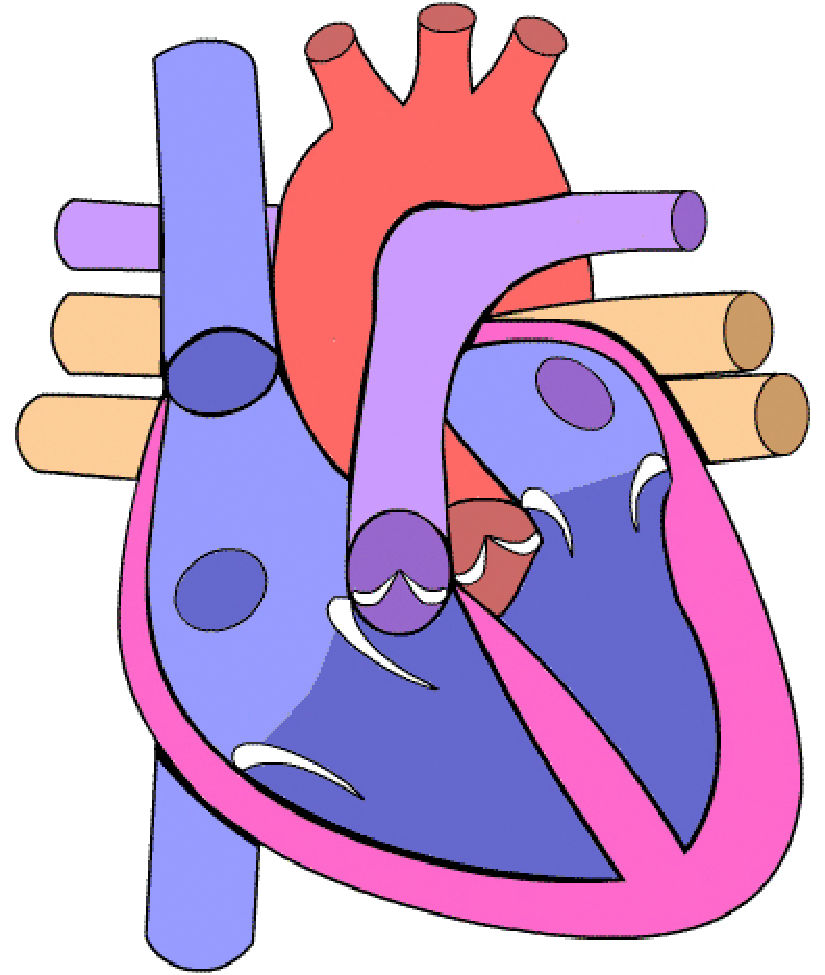
\includegraphics[height=6cm,keepaspectratio]{figure_12}}
		\caption{During rapid ventricular filling the atrioventricular valves open allowing blood to pass from the atria to the ventricles rapidly. The semilunar valves remain closed.}
		\label{fig:heart rapid ventricular filling}
	\end{subfigure}
	~
	\begin{subfigure}[t]{0.48\textwidth}
		\centering
		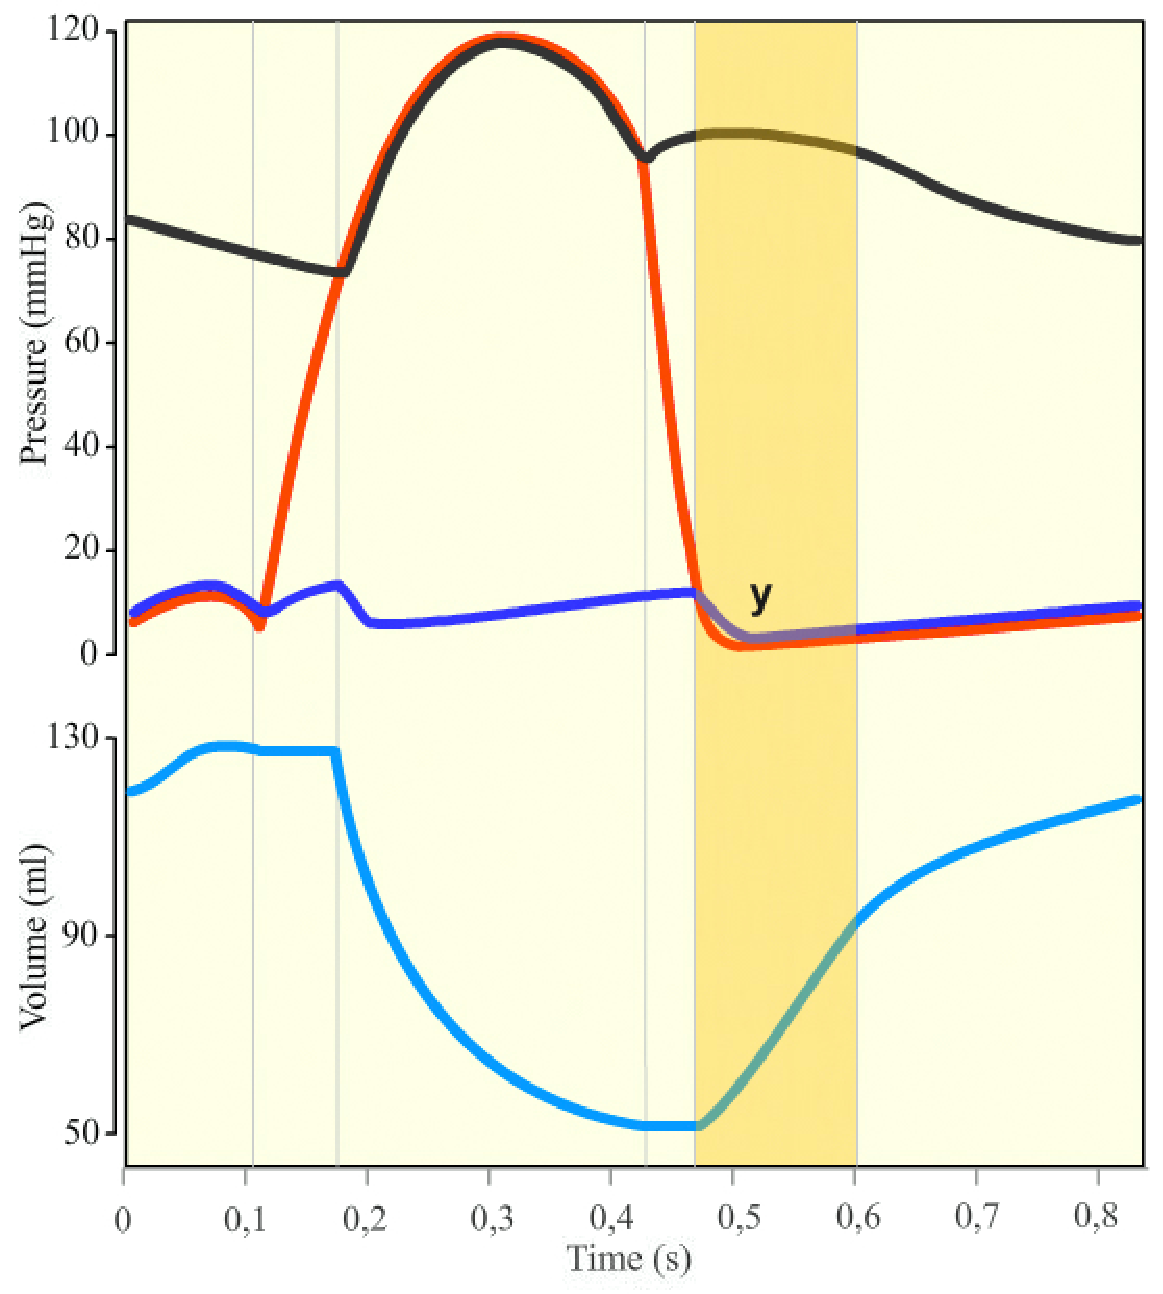
\includegraphics[width=\textwidth,keepaspectratio]{figure_13}
		\caption{Ventricular pressure is almost zero (red line) but the arterial pressure slowly decreases (black line). The atrial pressure (dark blue) reduces because of the blood flowing out of the atria. The blood volume in the ventricles (light blue) fill rapidly.}
		\label{fig:pressure rapid ventricular fillig}
	\end{subfigure}
	\caption[Rapid ventricular filling]{{Heart's mechanical changes, pressure and volume changes during rapid ventricular filling}}
\end{figure}

Also, the semilunar valves stay closed during this stage, but the arterial pressure starts to decrease slowly. In the arteries, the blood pressure never goes to zero as in the heart because of their recoil properties. Indeed, the minimum arterial pressure in the systemic circulation during a heart bit is commonly \SI{80}{\mmHg} which is known as diastolic pressure. In contrast, in the pulmonary circulations, the pressure could drop up to \SI{8}{\mmHg}. The electrical activity of the heart is null during this cycle. Hence, the isoelectric representation in the ECG wave.

\begin{figure}[!htpb]
	\centering
	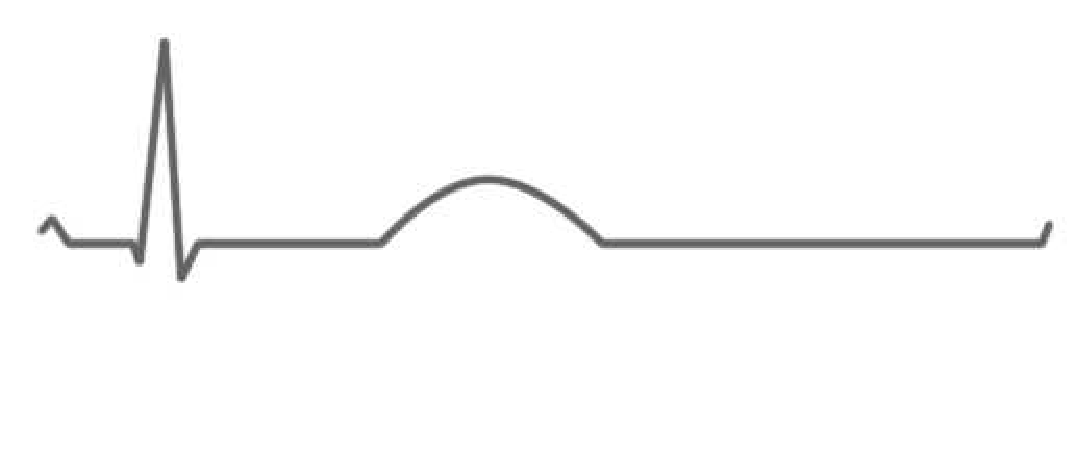
\includegraphics[width=0.5\textwidth,keepaspectratio]{figure_14} 
	\caption[ECG during rapid ventricular filling]{During rapid ventricular filling there is not electrical activity.}
	\label{fig:ECG rapid ventricular filling}
\end{figure}

\subsubsection{Slow ventricular filling}
In this stage, there is no change in the mechanical activity of the heart. Certainly, the valves remain the same as in the rapid ventricle cycle. The atrioventricular valves are open and the semilunar closed. Also, a small volume of blood goes into the ventricles, which come from the veins passing the atria and filling the ventricle slowly. The pressure in the ventricles still continues in zero, while the pressure in the atria slightly increases. The pressure in systemic and pulmonary circulation drops at a constant rate. 

In the heart's electrical path, at the end of the cycle, the depolarization moves away from the sino-atrial node to all around the heart producing the p wave showed in the ECG plot.  

\begin{figure}[!htpb]
	 \begin{subfigure}[t]{0.48\textwidth}
	 	\centering
	 	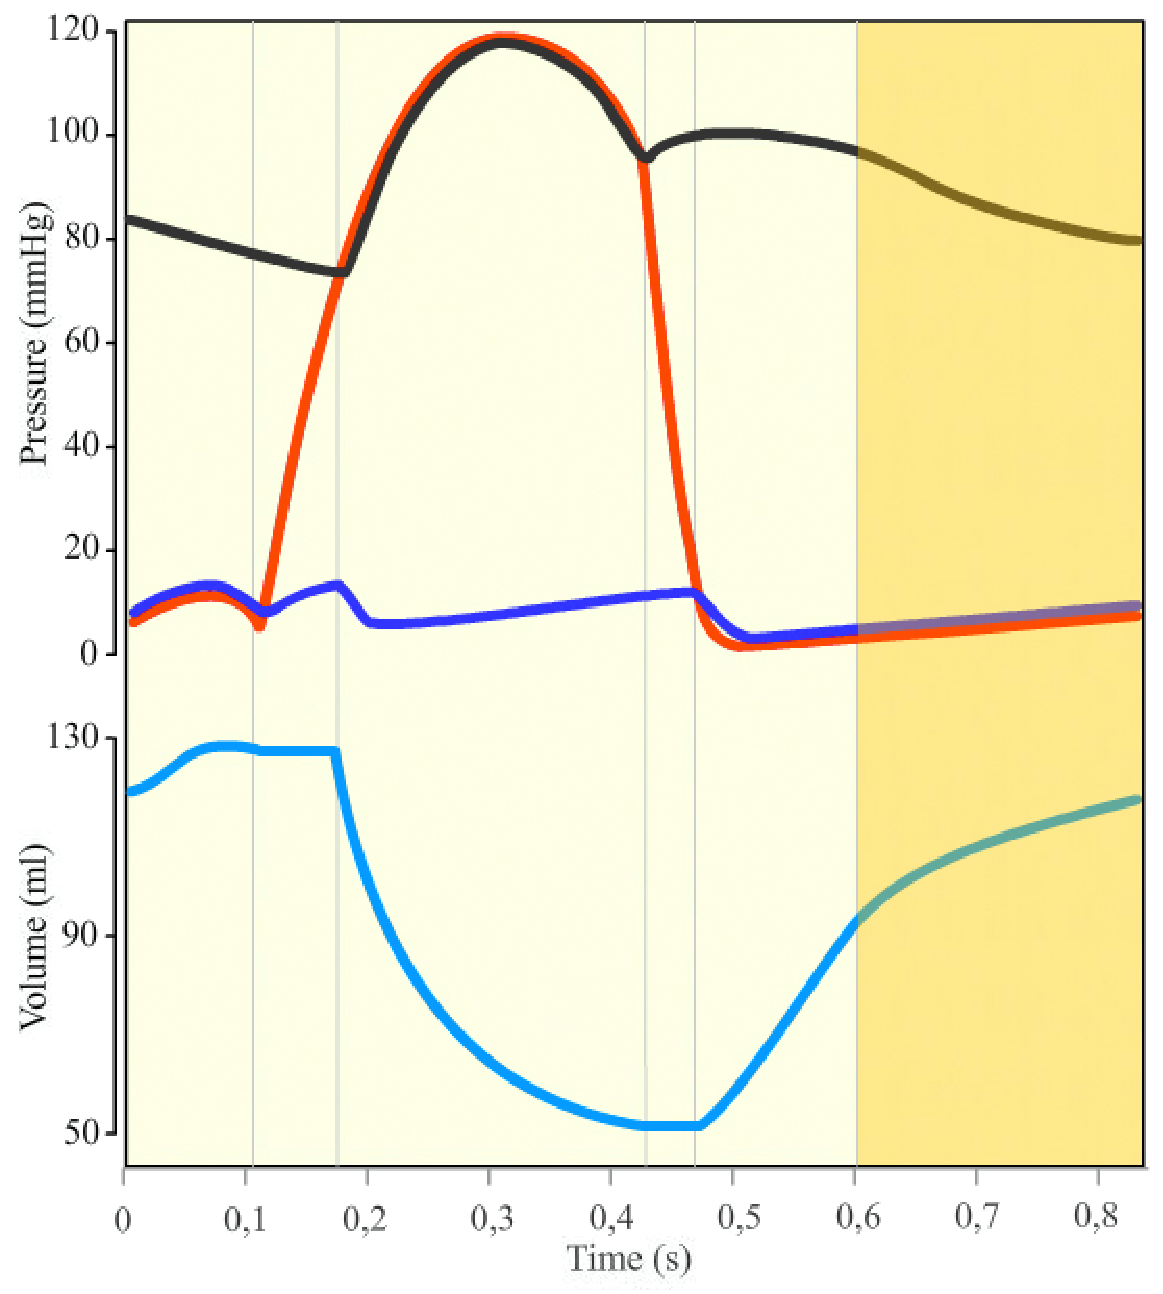
\includegraphics[width=\textwidth,keepaspectratio]{figure_15}
	 	\caption{Ventricular pressure continues almost in zero (red line). The arterial pressure slowly decreases (black line), as well as the atrial pressure (dark blue). The blood volume in the ventricles (light blue) fill slowly.}
	 	\label{fig:heart slow ventricular filling}
	 \end{subfigure}
	 ~
	 \begin{subfigure}[t]{0.48\textwidth}
	 	\centering
	 	\raisebox{2.75cm}{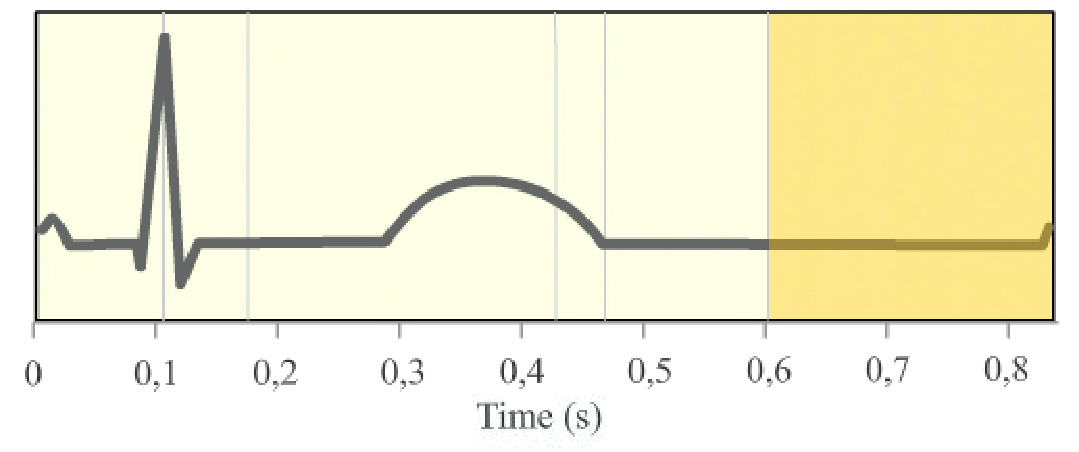
\includegraphics[width=\textwidth,keepaspectratio]{figure_16}}
	 	\caption{The depolarization of the heart spreads from the sino-atrial node. The P wave is visible in the waveform. }
	 	\label{fig:pressure slow ventricular fillig}
	 \end{subfigure}
	 \caption[Slow ventricular filling]{Pressures and volume during slow ventricular filling and ECG changes}
\end{figure}
 
\subsubsection{Atrial systole}
It is the last part of the cardiac cycle. In the mechanics of the heart during this phase, the ventricles fill entirely, while the atrioventricular valves open and the semilunar valves close. Also, an atrial contraction ejects blood from the atria to the ventricles. 

Thus, the atria eject approximately \SI{25}{\percent} of the ventricular filling volume to the ventricles. After that, the ventricular myocardium relaxes causing a light change of pressure in the ventricles, remaining close to zero. At the end of the atrial systole, the total blood volume in the ventricles is the end-diastolic volume about \SI{130}{\mmHg}. Due to the atrial contraction, there is a rise in the atria increasing the pressure of the chamber. It can be seen as the wave 'a' in the venous pulse in figure xxx. Finally, the arteries pressure continues decreasing constantly.

In the ECG waveform can be seen that the atrial depolarisation is completed and the end of the P wave is noticeable. During this phase, the depolarisation spreads from the atria to the atrioventricular node being possible the PR segment in the ECG.

\begin{figure}[!htpb]
	\begin{subfigure}[t]{0.48\textwidth}
		\centering
		\raisebox{1.25cm}{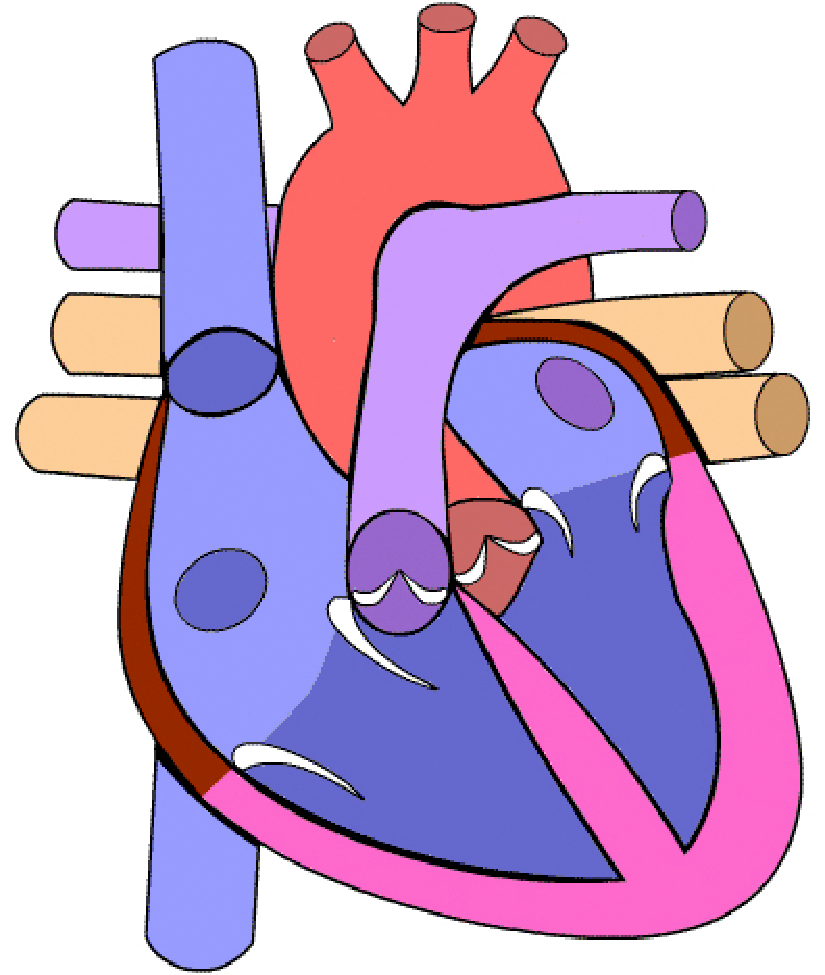
\includegraphics[height=6cm,keepaspectratio]{figure_17}}
		\caption{Ventricular pressure continues almost in zero (red line). The arterial pressure continue to decrease slowly (black line), there is a rise in the atrial pressure (dark blue). The ventricles are completely full (light blue) to end-diastolic volume (\SI{130}{\milli\litre}).}
		\label{fig:heart atrial systole}
	\end{subfigure}
	~
	\begin{subfigure}[t]{0.48\textwidth}
		\centering
		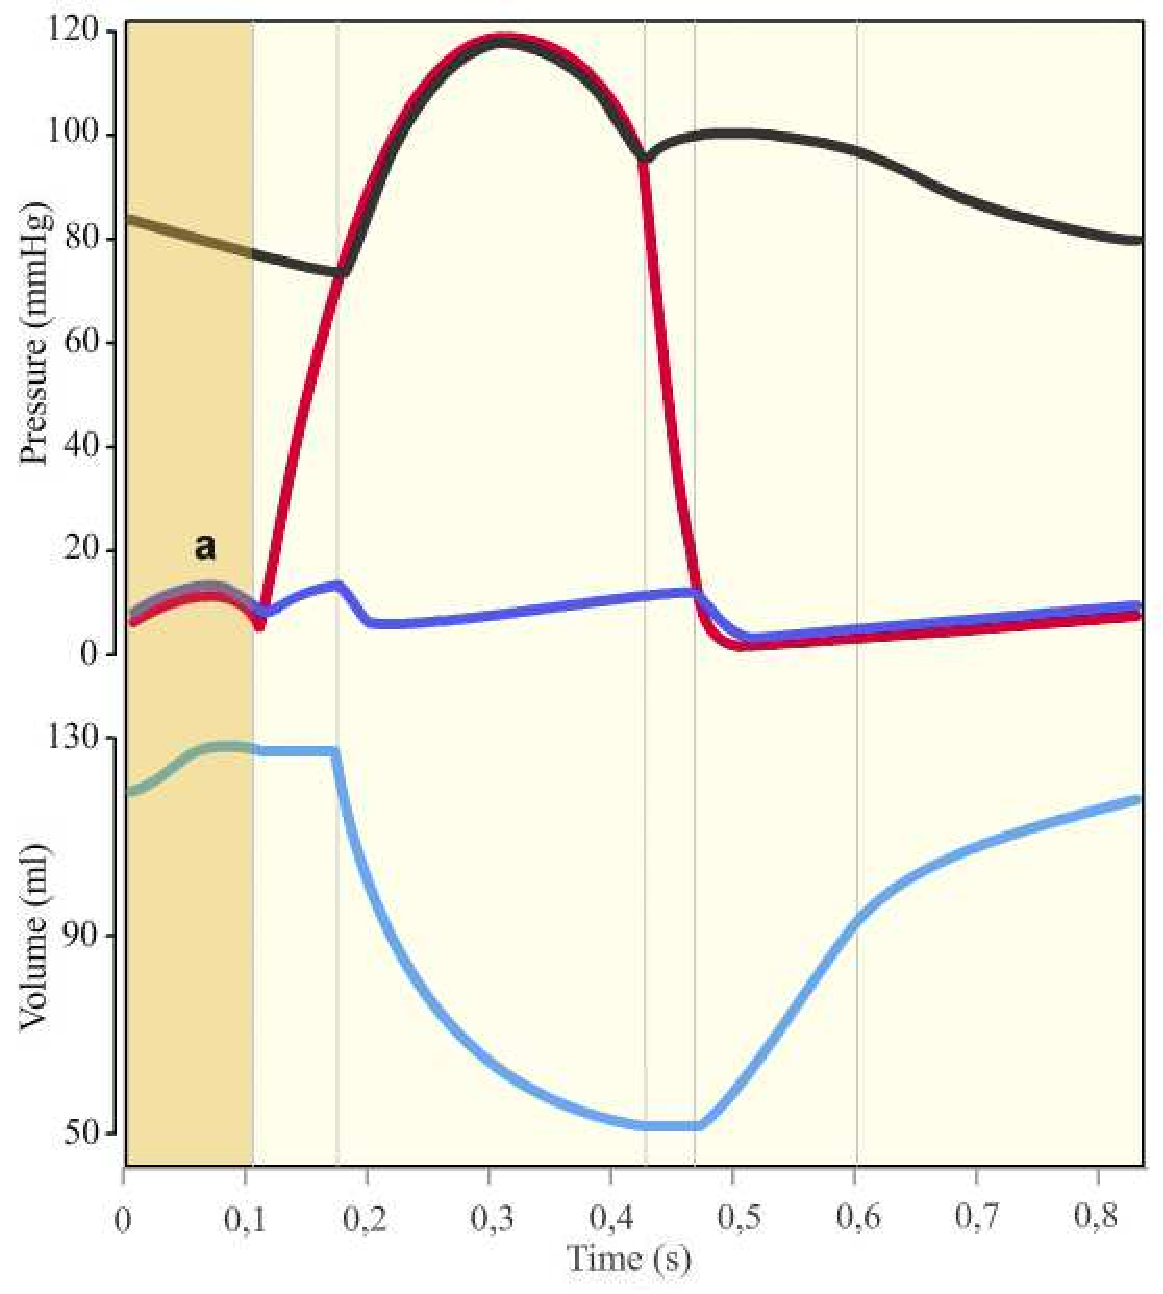
\includegraphics[width=\textwidth,keepaspectratio]{figure_18}
		\caption{The depolarization of the heart spreads from the sino-atrial node. The P wave is visible in the waveform. }
		\label{fig:pressure atrial systole}
	\end{subfigure}
	\caption[Slow ventricular filling]{Pressures and volume during slow ventricular filling and ECG changes}
\end{figure}

\begin{figure}[!htpb]
	\centering
	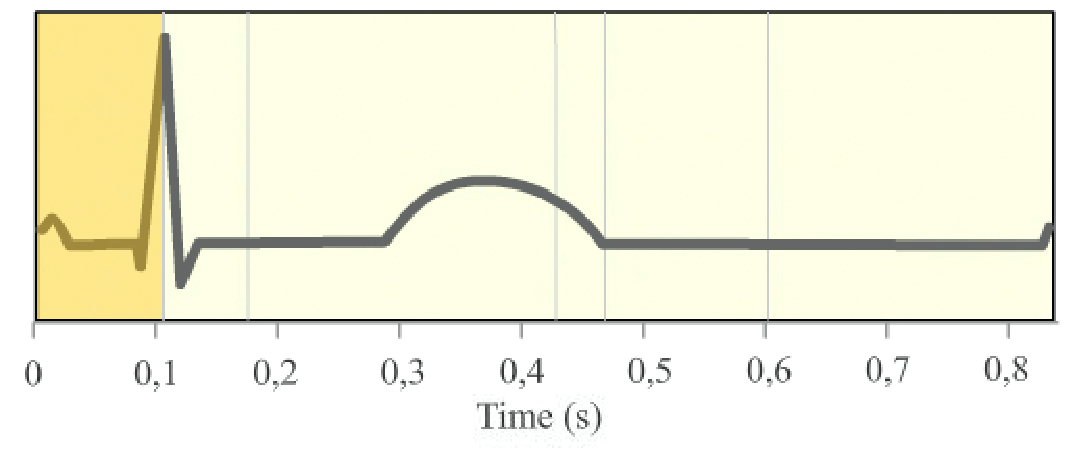
\includegraphics[width=0.5\textwidth,keepaspectratio]{figure_19} 
	\caption[ECG during rapid ventricular filling]{During rapid ventricular filling there is not electrical activity.}
	\label{fig:ECG atrial systole}
\end{figure}
 
\section{Upper limb anatomy}
The experimental work of this document described in chapter \ref{chapter procedure} was carried out in the forearm. This section describes the anatomy of the upper arm and the forearm. This information helps to understand the position of the electrodes and the nearby tissue that interacts with the impedance plethysmography device. 

The arm is part of the upper limb of the human anatomy. It divides into three sections, the upper arm, the forearm and the hand. The following description corresponds to the upper arm and forearm as are the parts involve in the study. The upper arm is the section between the shoulder and the elbow and the forearm from the elbow to the wrist. 


\subsection{Bones of the arm}
Figure \ref{fig:upper limb bones} shows the bones of the upper arm, the humerus is the only bone in this part of the arm. This bone connects the scapula to the radius and ulna which are the bones that make part of the forearm. These bones connect to the carpus bones in the hand which composes the wrist. The rest of the hand's bones are the metacarpus and the phalanges. 

\begin{figure}[!htpb]
	\centering
	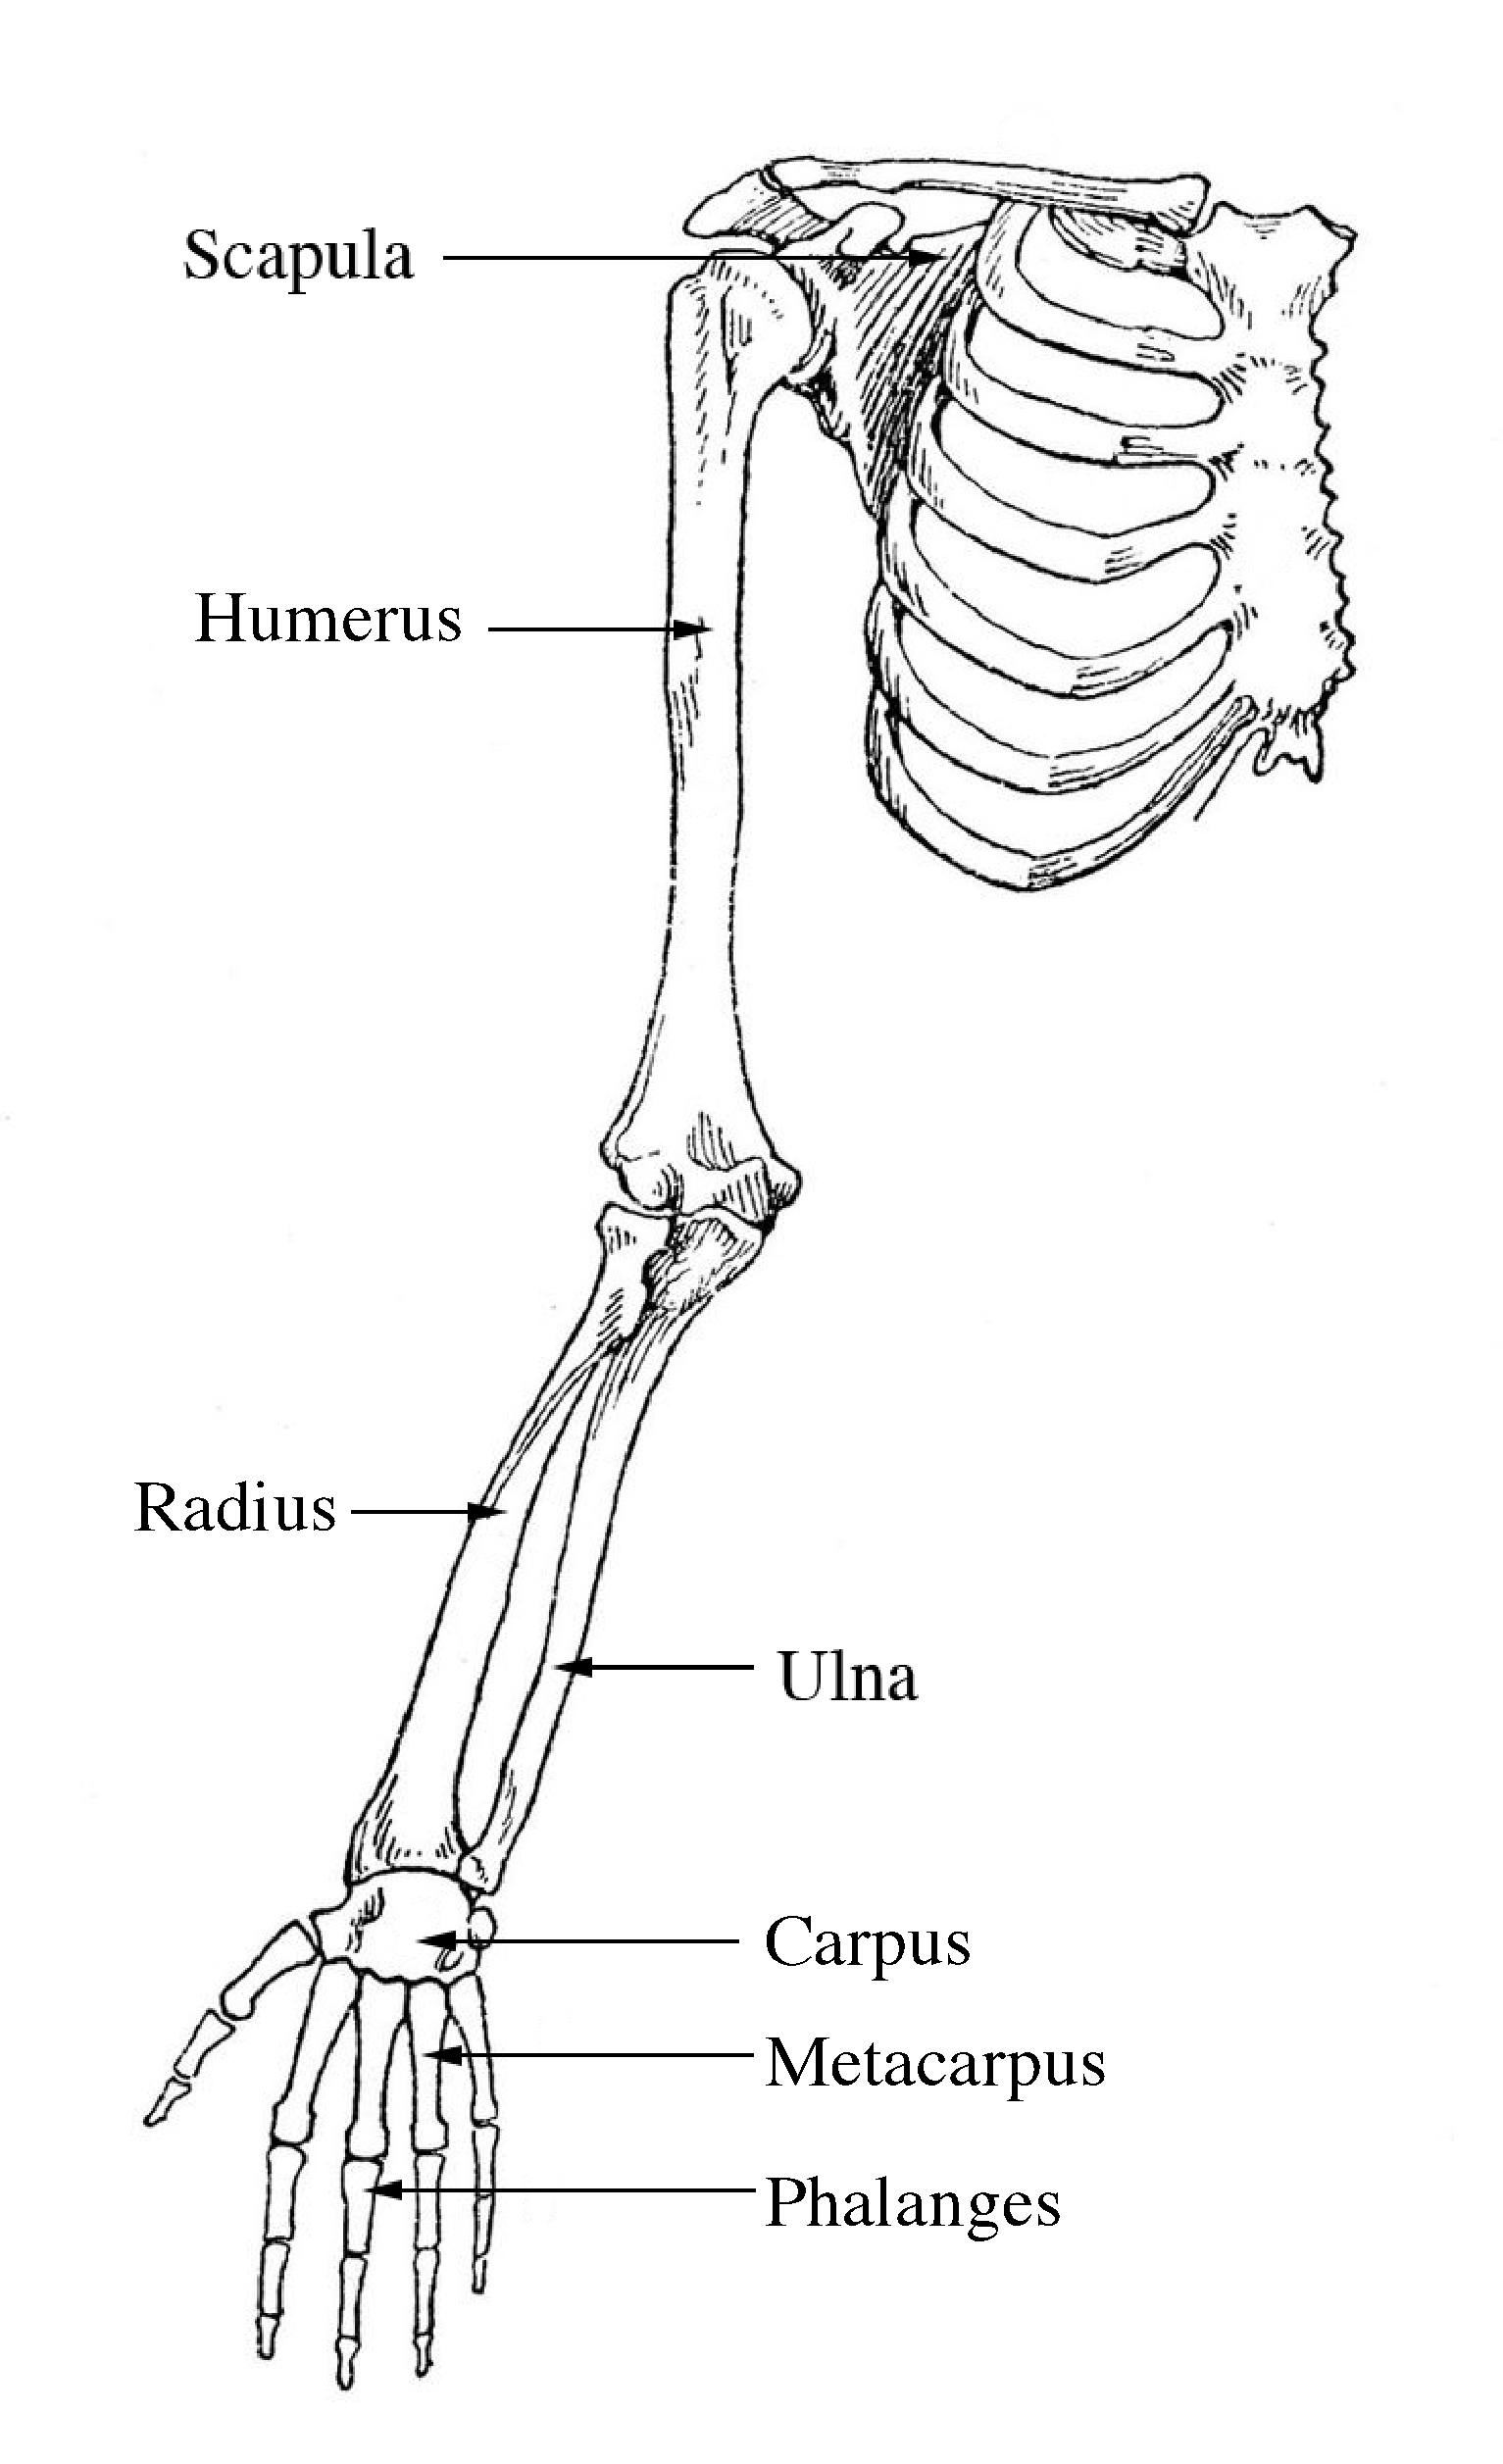
\includegraphics[width=0.4\textwidth,keepaspectratio]{figure_20} 
	\caption{Bones of the upper arm}
	\label{fig:upper limb bones}
\end{figure}


\subsection{Muscles of the arm}
The muscles of the arm are divided by a fascial layer called lateral and intermuscular septa. These sections of the muscles are known as anterior (see figure \ref{fig:upper arm anterior}) and posterior compartments (see figure \ref{fig:upper arm posterior}). The upper arm contains four muscles. In the anterior compartment the biceps brachii, brachialis and coracobrachialis, and in the posterior compartment is the triceps brachii. 

\begin{figure}[!htpb]
	\begin{subfigure}[t]{0.52\textwidth}
		\centering
		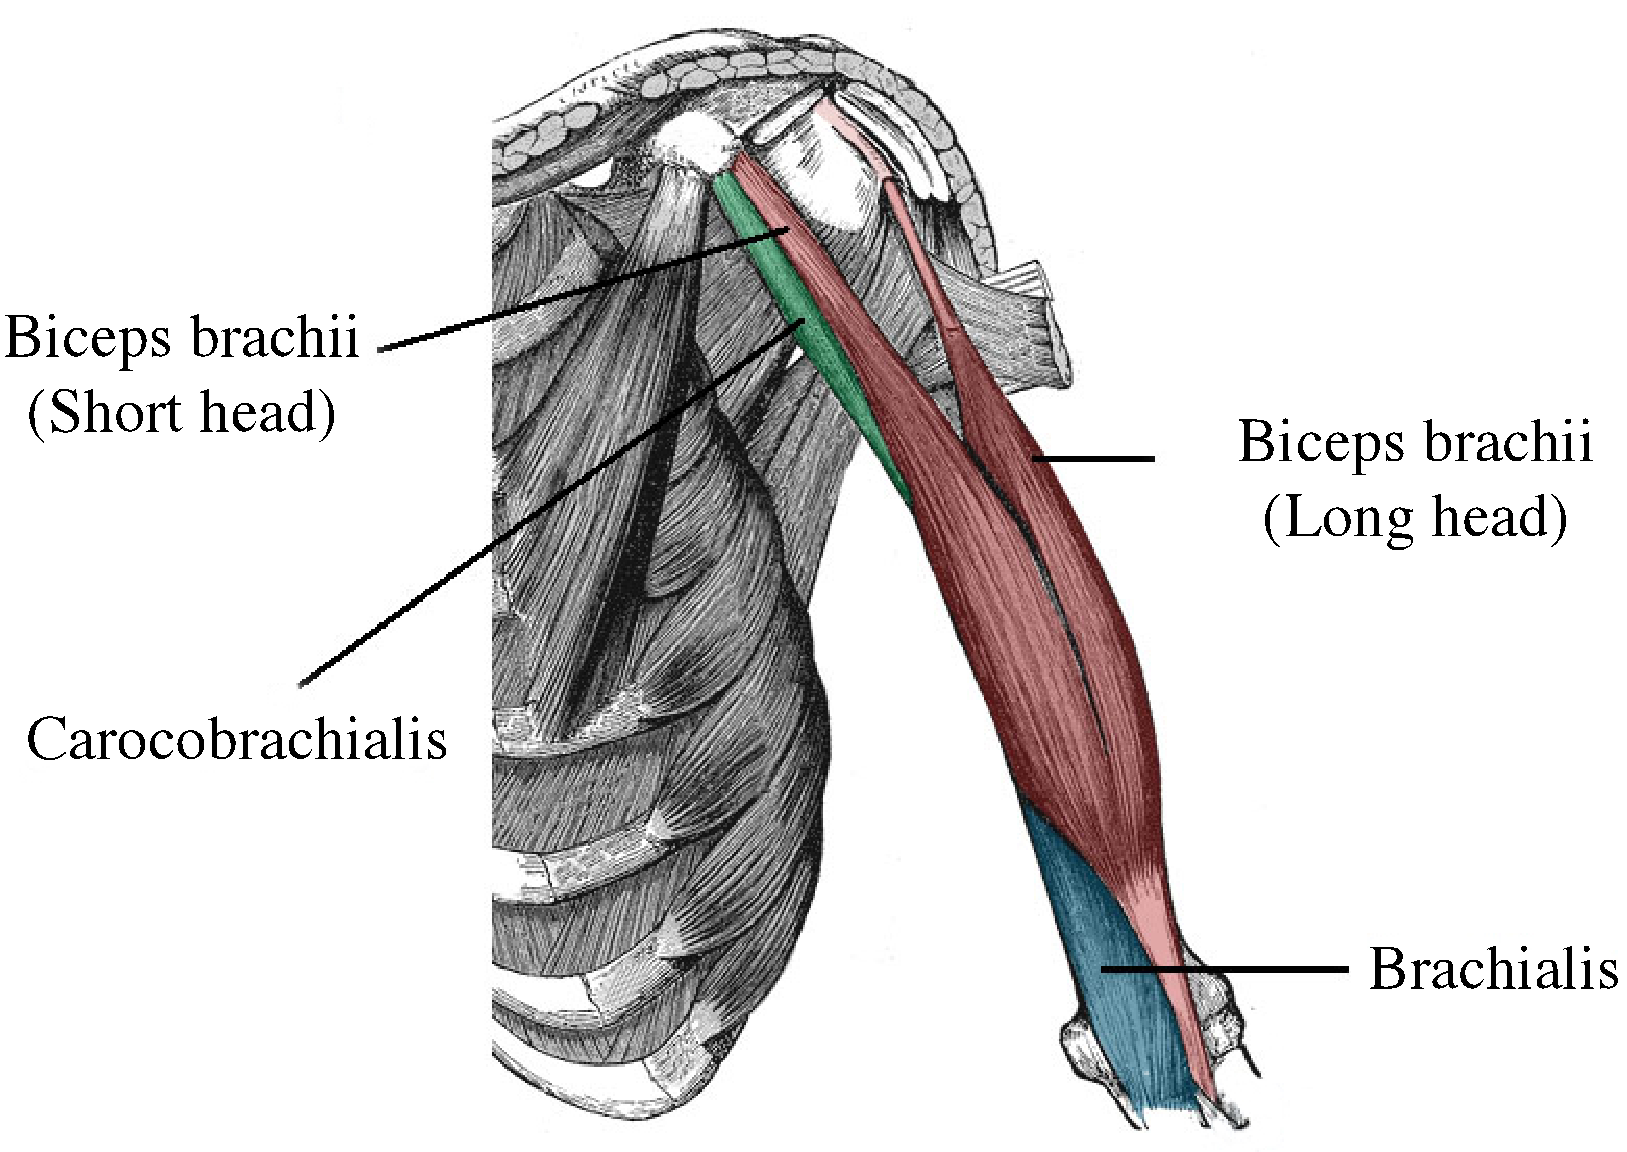
\includegraphics[height=5.5cm,keepaspectratio]{figure15a}
		\caption{Muscles of the anterior compartment}
		\label{fig:upper arm anterior}
	\end{subfigure}
	~
	\begin{subfigure}[t]{0.44\textwidth}
		\centering
		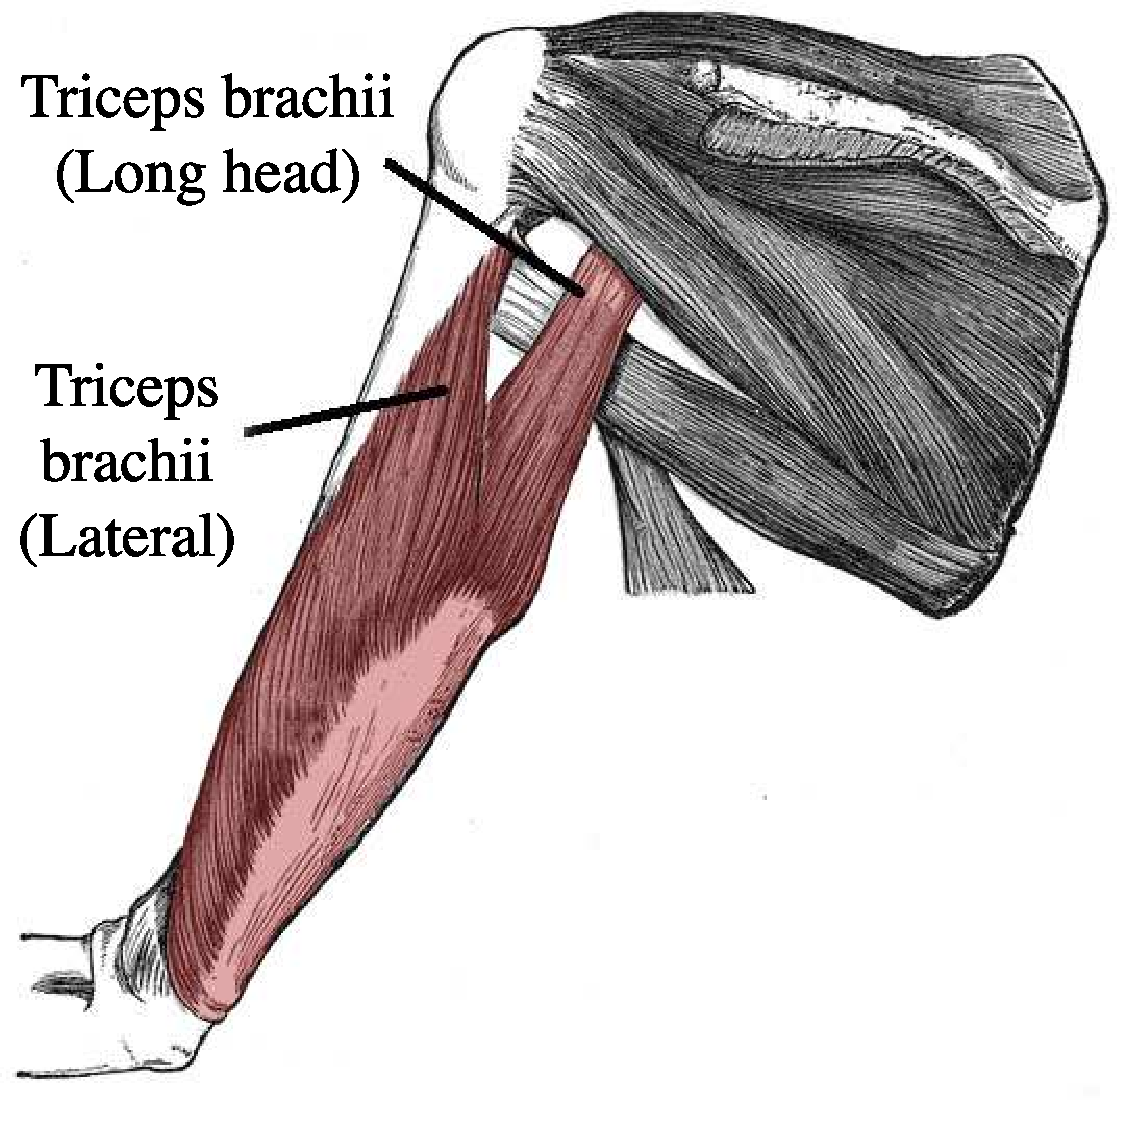
\includegraphics[height=5.5cm,keepaspectratio]{figure15b}
		\caption{Muscles of the posterior compartment}
		\label{fig:upper arm posterior}
	\end{subfigure}
	\caption{Muscles of the upper arm}
\end{figure}

The forearm is composed of many muscles that perform flexion of the wrist and fingers, as well as pronation.  In the anterior compartment is divided into three kinds; superficial, intermediate and deep. In the superficial compartment are located the flexor carpi ulnaris, palmaris longus, flexor carpi radialis and the pronator teres. The only muscle of the intermediate compartment is the flexor digitorum superficialis. All these muscles are shown in figure \ref{fig:forearm anterior},

\begin{figure}[!htpb]
	\centering
	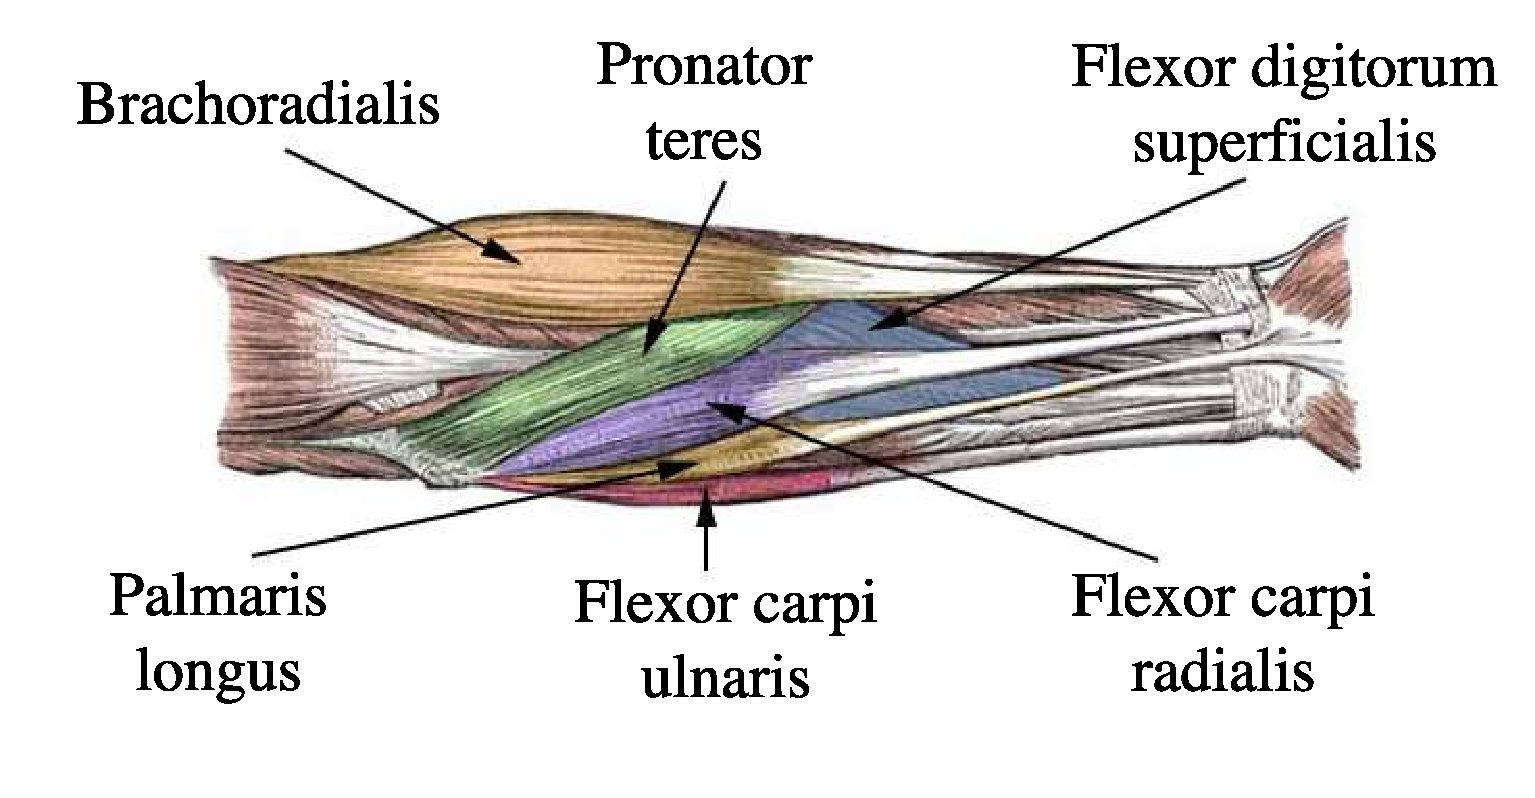
\includegraphics[height=4.5cm,keepaspectratio]{figure16}
	\caption{Muscles of the anterior compartment}
	\label{fig:forearm anterior}
\end{figure}	

Finally, as shown by figure \ref{fig:forearm deep} in the deep compartment are located three muscles, the flexor digitorum profundus, flexor pollicis longus and the pronator quadratus.

\begin{figure}[!htpb]
	\centering
	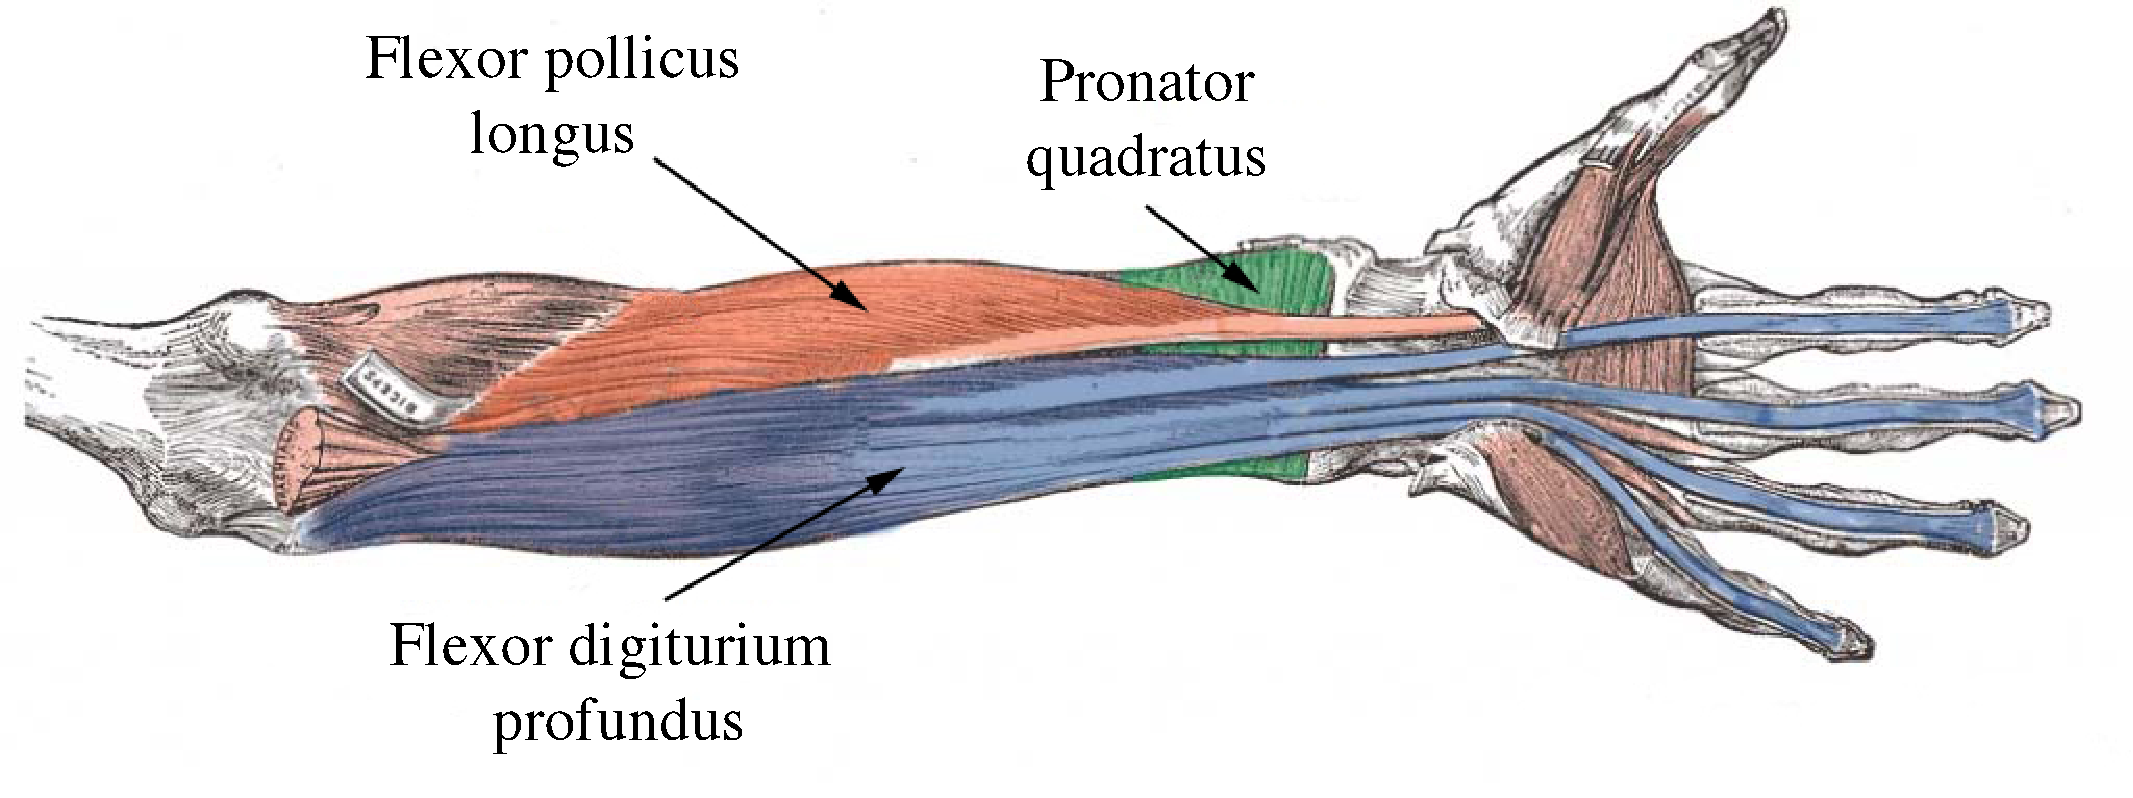
\includegraphics[height=4.5cm,keepaspectratio]{figure17}
	\caption{Muscles of the deep compartment}
	\label{fig:forearm deep}
\end{figure}

\subsection{Circulation of the arm}
\subsubsection{Arterial circulation}
The subclavian arteries located in the chest area supply the blood of the arm.  The right arm blood supply comes from the right subclavian artery which is attached to the brachiocephalic trunk (see figure \ref{fig:subcalvian}). In contrast, the blood supply of the left arm comes directly from the subclavian artery connected to the arch of the aorta. 

\begin{figure}[!htpb]
	\centering
	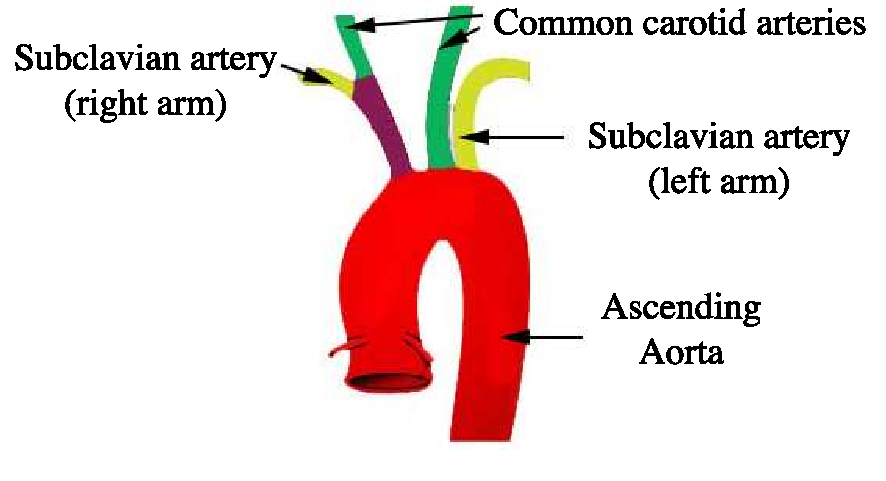
\includegraphics[height=4.5cm,keepaspectratio]{figure18}
	\caption{Origin of the subclavian arteries}
	\label{fig:subcalvian}
\end{figure}

When these arteries pass through the axilla, they are known as axillary arteries. From this artery, other arteries arise such as the posterior and anterior circumflex arteries which supply blood to the shoulder section, and the subscapular artery which is the largest. 

Hereafter, as shown in figure \ref{fig:upper arm circulation} the axillary artery becomes the brachial artery at the teres major muscle, which is the blood supply for the whole arm.  From this artery, other arteries arise that supply blood to the tissues in the upper arm. Such as the profunda brachii which is the deep artery of the arm travelling around the posterior surface of the humerus. 

\begin{figure}[!htpb]
	\centering
	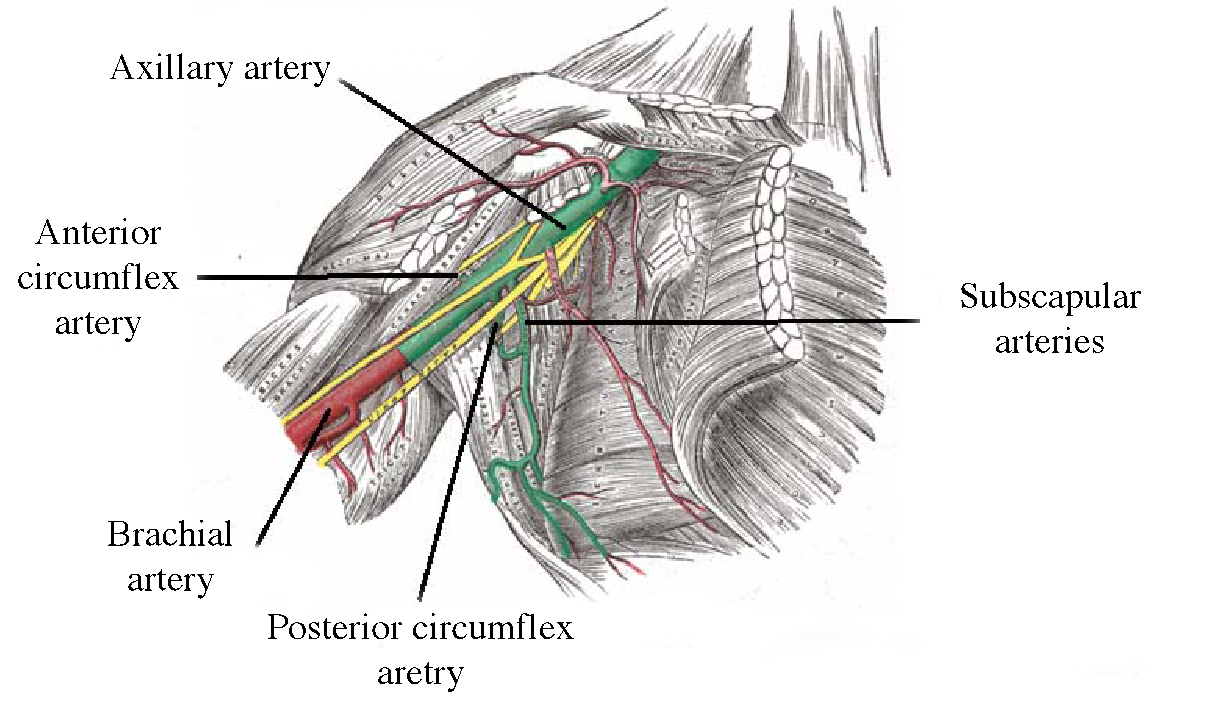
\includegraphics[height=6cm,keepaspectratio]{figure19}
	\caption{Origin of the subclavian arteries}
	\label{fig:upper arm circulation}
\end{figure}

As it can be seen in figure \ref{fig:forearm aretries}, as soon as the brachial artery passes the cubital fossa (front of the elbow joint) underneath the brachialis muscle, this artery bifurcates becoming the radial and ulnar arteries. The radial artery supplies blood to the posterior tissues of the arm and the ulnar to the anterior. At the carpus bones, these arteries anastomose in the hand forming the superficial and deep palm arches which provide blood to the different tissues located in the hand. 

\begin{figure}[!htpb]
	\centering
	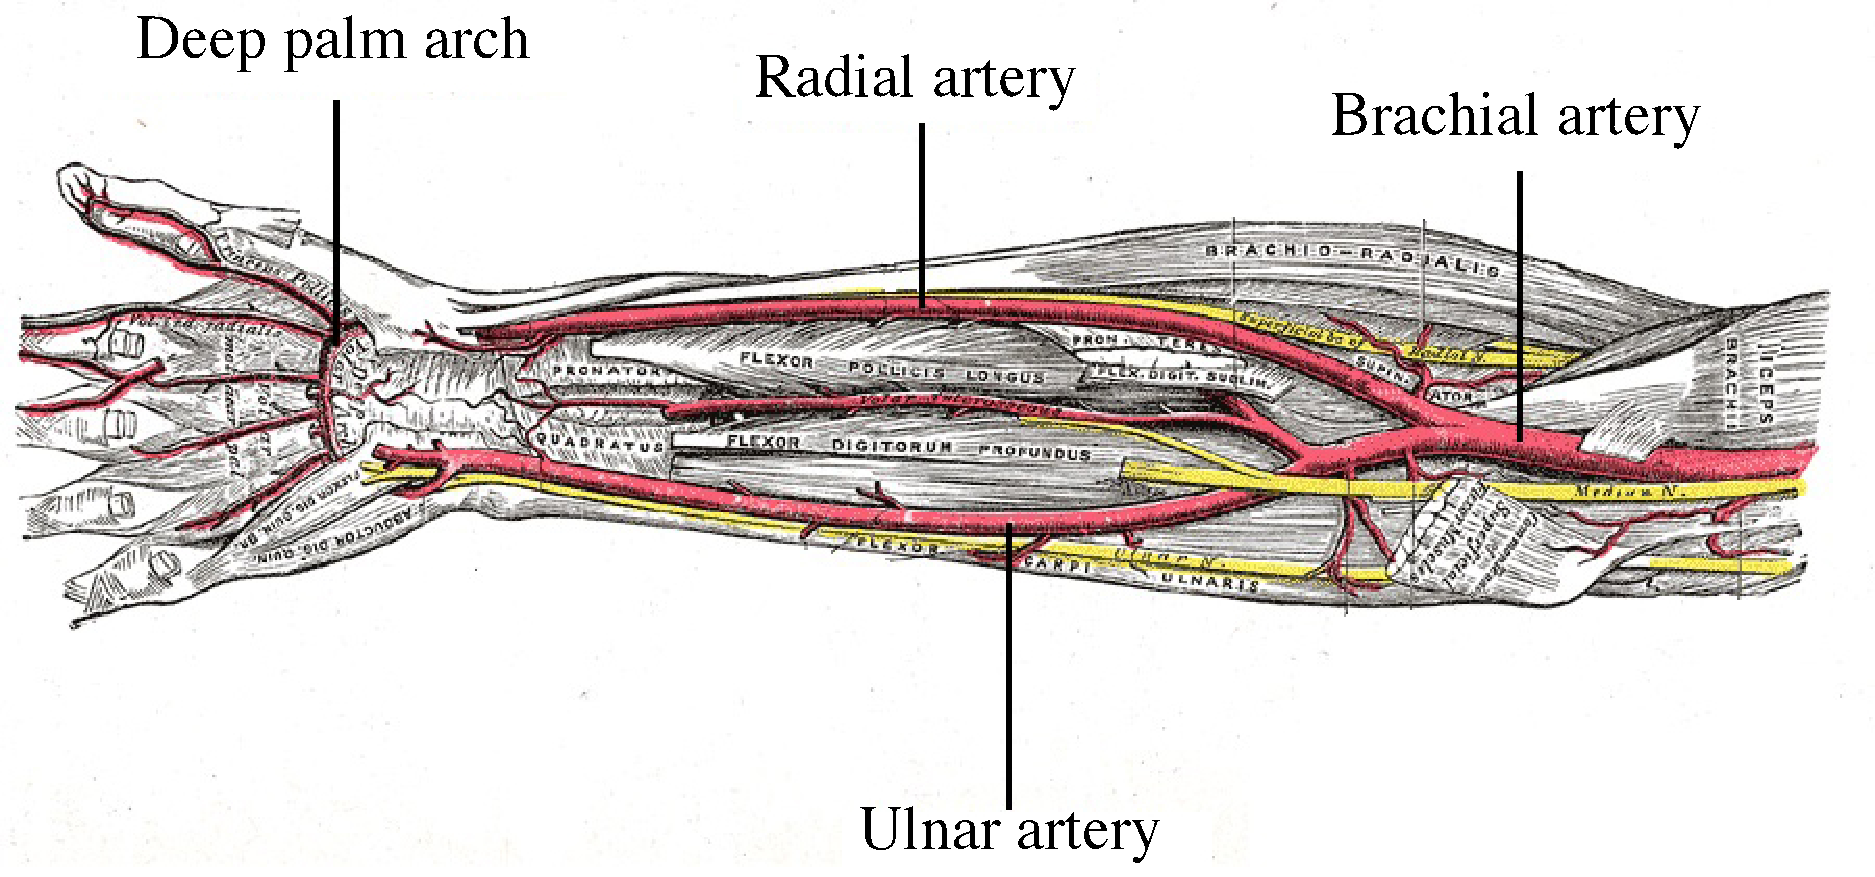
\includegraphics[height=4.5cm,keepaspectratio]{figure20}
	\caption{Forearm arteries}
	\label{fig:forearm aretries}
\end{figure}

\subsubsection{Venous circulation}
The venous of the arm are anatomically split into the superficial and the deep veins (see figure \ref{fig:arm veind}). The greatest superficial veins in the upper limb located subcutaneously are the cephalic and basilic veins. The latter originates at the venous branches of the hand, near the teres major the vein goes deep into the arm. At this point, this vein combines with the brachial veins to form the auxiliary vein. 

The cephalic vein begins at the dorsal venous network of the hand. It ascends on the anterolateral region of the arm and at the elbow passes to the anterior part of the limb. In this same section, the median cubital vein connects the cephalic and basilic veins. At the axilla, the cephalic vein joins to the axillary vein. 

The deep fascia contains the deep veins in the upper limb. These veins are paired to either side of the brachial, radial and venous artery. Hence, they inherited the same names.  In fact, the pulsation of the brachial artery helps the venous return of the arm. This effect is known as vena comitantes. The perforating veins connect the deep and superficial veins of the upper arm. 

\begin{figure}[!htpb]
	\centering
	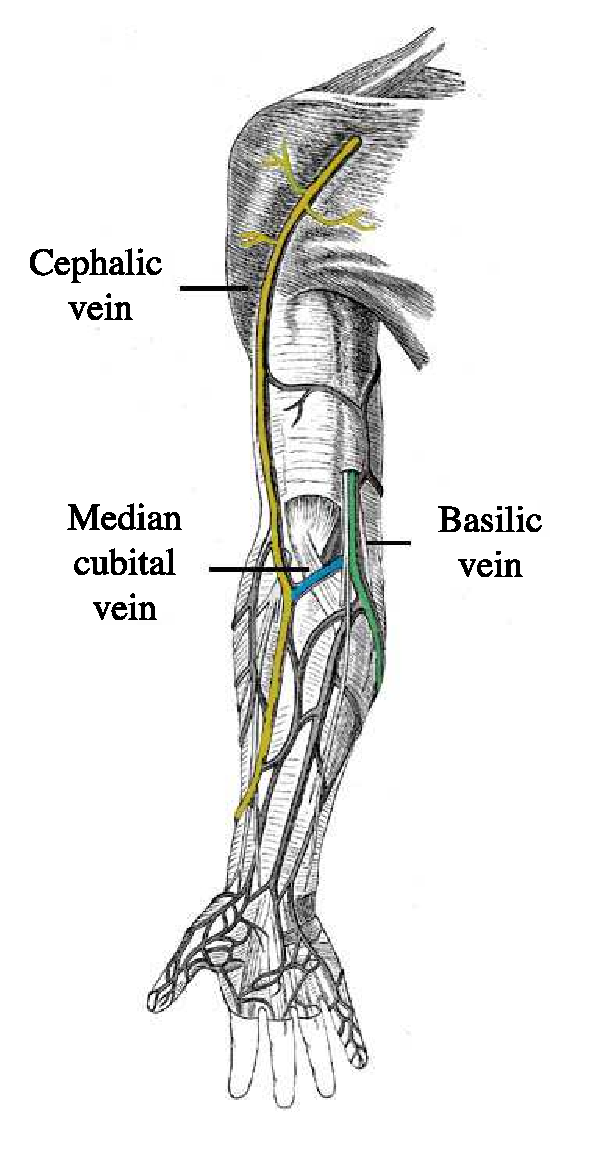
\includegraphics[height=10cm,keepaspectratio]{figure21}
	\caption{Forearm arteries}
	\label{fig:arm veind}
\end{figure} 

%********************************** %Section 2.1.2  **************************************
\section{Oxygen transportation}
\label{section literature 1.2}
Oxygen ($O_2$) is an essential component needed by all body's cells to complete metabolic processes. Within the blood, this is transported by haemoglobin (Hb) contained within red blood cells (RBCs). Oxygen is required for the chemical reactions needed to convert biochemical energy from nutrients coming from food into cell's energy known as coenzyme or adenosine triphosphate (ATP). As a result of this reaction waste product is released from the cell. A human cell can only survive for a few minutes without oxygen~\cite{culmsee2005apoptosis}.

Inadequate oxygen delivery to body's tissue is known as hypoxia. There are different classifications of hypoxia count based on its cause~\cite{marieb2007human} which are described as follows: 

\begin{enumerate}
    \item \textbf{Anaemic Hypoxia:} It is a condition where a body part or an organ has poor $O_2$ delivery. Some of the causes are a small count of RBCs and abnormal or too little Hb content in the blood's cells.
    \item \textbf{Ischemic (stagnant) hypoxia: }This is caused when blood circulation is reduced or blocked. There are different causes for this. However, the most commons are congestive heart failure that may cause body–wide hypoxia, emboli or thrombi blocking oxygen supply to the tissue distal from the occlusion. 
    \item \textbf{Histotoxic hypoxia: }Mainly caused by metabolic poisoning like ingestion of cyanide. In this case the cell is unable to use $O_2$ for metabolic purposes, even though there is an appropriate amount of $O_2$ being delivered by the body.
    \item \textbf{Hypoxemic hypoxia:} It is shown by a decrease in the arterial oxygen partial pressure ($PO_2$). Some of the causes are an imbalance in the ventilation–perfusion coupling mechanism, poor ventilation caused by pulmonary disease and breathing air with a low content of $O_2$. Moreover, carbon monoxide ($CO$) poisoning is another reason behind this illness because it has \num{200} times more affinity with Hb than $O_2$. Thus, in places with high concentration of CO such as fires could lead easily to death.
\end{enumerate}




%********************************** %Section 2.2  **************************************
\subsection{Problems derived from poor blood delivery} %Section 2.3
\label{section literature 3}
Now that has been described some of the problems of having a poor oxygen transportation of blood at a cellular level; more detail will be unveiled about illnesses due to the poor or total lack of blood delivery to human tissue especially human limbs. 

Ischemia develops when there is an insufficient supply of blood to an organ. For instance, if an artery blockage occurs all the tissue below the path will suffer from starvation of oxygen and other critical nutrients. Different causes could lead to the blockage of an artery which can be caused by external or internal factors. Speaking specifically of lower limbs, these represent a significant cause of disability and cardiovascular morbidity and mortality~\cite{novo1995patients}. 

Exists different kind of diseases compromising limbs, an example of this is peripheral arterial disease (PAD), which also originates in another kind of illnesses according to the kind of occlusion or blockage. For instance, critical limb ischemia (CLI), which is a condition where as a consequence of arterial disease, a patient experiments pain in the extremity even at rest or in a breakdown of the skin~\cite{novo2004critical}. 

Clinically there are different forms to assess the development of this illness. Some scales of qualitative evaluation have been developed such as the Rutherford classification, the Leriche-Fountaine classification or the TACS II classification of femoral and popliteal lesions~\cite{norgren2007inter}. Health practitioner uses a survey, an indicator of pain when walking and a visual inspection is possible to determine the stage or the severity of the arterial occlusion.  Table \ref{table:Fountaine}) shows the different stages of the Leriche-Fountain classification and the various steps considered to evaluate the illness.

\begin{table}
\caption{Leriche-Fountaine classification}
\centering
\label{table:Fountaine}
\begin{tabular}{p{1.8cm} p{3.8cm} p{3.5cm} p{4.5cm}}
\toprule
\textbf{Stages}& \textbf{Symptoms} & \textbf{Pathophysiology} & \textbf{Pathophysiological \newline classification} \\
\midrule
Stage I & Asymptomatic \newline or effort pain & Relative hypoxia & Silent Arteriopathy \\
\midrule
Stage II A & Effort pain \newline Pain free walking distance > \SI{200}{\meter} & Relative hypoxia & Stabilized Arteriopathy \newline Non-Invalidant claudication \\ 
\midrule
Stage III A & Rest Pain \newline Ankle arterial pressure > \SI{50}{\mmHg} & Cutaneous hypoxia \newline Tissue acidosis \newline Ischemic neuritis & Instable arteriopathy \newline Invalidant claudication \\
\midrule
Stage III B & Rest pain \newline Ankle arterial pressure < \SI{50}{\mmHg} & Cutaneous hypoxia \newline Tissue acidosis \newline Ischemic neuritis & Instable arteriopathy \newline
Invalidant claudication \\
\midrule
Stage IV & Trophic lesions \newline Necrosis or Gangrene & Cutaneous hypoxia \newline 
Tissue acidosis & Necrosis \newline Evolutive arteriopathy \\
\bottomrule
\end{tabular}
\end{table}

As table~\ref{table:Fountaine} shows, there are various levels of stratifying the severity of the disease according to the symptoms that are related pathophysiology. According to the gravity of the stage where the patient is, there are different methods to examine the severity of the disease using imaging methods. These will be described in detail in the section xxx.

\mynote{relate this to a section in the document later on}

There are a significant number of illnesses that are derived from the inadequate delivery of blood towards a limb. According to their physiology, they can be divided into a disease which affects either the microcirculation or main vessels or both. The following are just an example of the different diseases that may require continuous blood flow monitoring in acute or chronic settings.



%********************************** %Section 2.2.1  **************************************
\subsubsection{Peripheral vascular disease}
\label{section literature 2.1}
Some of the common forms of reduction in blood towards a limb are known as the peripheral vascular disease (PVD) also known as peripheral arterial disease (PAD). This sickness is a progressive vascular condition caused by the blockage, narrowing, or spasms in a blood vessel (arteries, veins or lymphatic vessels). Hence, altering the blood circulation to and from any upper or lower extremities.  Most commonly affect the lower limbs, especially legs and feet. Therefore, the derivation of its name as "peripheral" because it affects mostly the periphery of the body. It affects \SI{5}{\percent} of people over \num{50} and between \SIrange{12}{20}{\percent} of people over 65 years old. To some extent, it is more common in men than women. People with certain risk factors are more likely to suffer PVD such as patients with diabetes of smokers.  

\mynote{I need a reference for this numbers}

Different factors could cause the narrowing of the blood vessels. The most common cause of PVD is atherosclerosis, deposition of fatty material on the arterial walls. This fatty material constitutes a plaque that reduces the blood flow towards tissue in the limb lessen the transport of $O_2$ and nutrients as explained in Oxygen transportation section. Moreover, clots may also form on the artery walls reducing the internal size of the vessel and increasing the risk of obstructing off a major artery. 

Different risk factors are contributing to the development of this sickness. Some can be inherited to the population others are based on lifestyle choices. The combination of two of more of the following risks may increase complications from PVD, such as smoking and diabetes. However, more in details some of the documented risk factors are:

\begin{itemize}[noitemsep]
    \item Age (especially over \num{50})
    \item Family history (high blood pressure, high cholesterol or PVD)
    \item Diabetes
    \item Smoking
    \item Obesity
    \item Infections
    \item Coronary artery disease
    \item Injury to vessels
    \item Physical inactivity
    \item High blood pressure
    \item Autoimmune diseases
    \item Nutritional deficiencies
    \item High blood cholesterol
    \item Emboli from other locations in the body
    \item Inflammation of the blood vessels
\end{itemize}

On the first stages of the illness, symptoms are not noticeable, which makes difficult to diagnose the condition. Just until it has been developed into a painful stage as described by the Fountaine's classification (see table \ref{table:Fountaine}) is when actions come into place. However, performing a qualitative assessment of the extremity helps to diagnose the sickness in early stages. Some of the indicators could be coldness to touch, poor skin condition (thinning, shining or brittle), poor nail health (thickening or opaque nails), hair loss in the extremity, reduced pulse sensation in the extremity, impotence, infections or injuries not healing properly, poor muscle condition (numbness, weakness or heaviness), pain while walking and stop at rest, local skin discolouration (pale, blue or dark red) and restricted mobility. 

Once a qualitative or physical examination has been performed, and the progress of the illness has been classified there are additional tests that may help to diagnose the severity of the PVD. Some of the methods just require the assessment of the medical practitioner using common medical devices others may need the use of specialised equipment. Some of the therapeutic methods that do not demand the use of bulky or cumbersome devices are:

\begin{itemize}
    \item \textbf{Ankle-branchial index (ABI):} It is the ratio of the differential measurement of systolic blood pressure measured at the ankle to that measured at the brachial artery [17]. For this it is required to compared the difference in blood pressure between the arm and the ankle, it also needed to record the ankle's blood flow using a Doppler ultrasound instrument.  
    \item \textbf{Treadmill exercise test: }In this method the patient has to walk or run to monitor the circulation during exercise. Pain or problems during the test are recorded to examine the severity of the obstruction.
    \item \textbf{Reactive hyperaemia test:} This test refers to a temporary increase (\textit{hyper}) of blood flow (\textit{emia}) of the extremity. It is usually performed in people who are not able to walk on a treadmill. In this case, the person is taken to supine position and comparative measurements of blood flow in tights and ankles are taken after occlusion to determine any decrease between both sites. 
\end{itemize}

%********************************** %Section 2.2.2  **************************************
\subsubsection{Compartment syndrome}
\label{section literature 2.2}                                                                                                                                                                                                                                                                                                                                                                                                                                                                                                                                                                                                                     
All the muscles, blood vessels and nerves are contained within a tissue known as fascia. When the pressure in a limb within this compartments increases because of bleeding or swelling, it could lead to total or partial restriction of micro–vascular blood flow \cite{songer2001tissue}. Some cases may present rapid discolouration and blistering of the affected limb being commonly associated with oedema, cyanosis and severe pain \cite{chhabra2013compartment}. Hence, it can lead ultimately to venous hypertension and loss of blood plasma. If the arterial flow is reduced, it also may result in gangrene, limb loss or even death \cite{lamborn2014compartment}. This syndrome can be catalogued as acute when is caused by either an injury, accident or medical emergency, and chronic when occurs gradually during any sports activity.

The most common method to diagnose this illness is Doppler sonography \cite{chhabra2013compartment}. Nevertheless, detecting foot compartment syndrome could be challenging compared to other parts of the body because its symptoms and indicators are less reliable \cite{dodd2013foot}.

%********************************** %Section 2.2.3  **************************************
\subsubsection{Diabetic foot infection}
\label{section literature 2.3} 
The lack of blood towards an extremity can also be caused by a secondary effect of other illness like diabetes. Some of the most common problems that diabetic patients have to deal with are diabetic foot infection which is a clinical syndrome characterised by local findings of inflammation or purulence in a person with diabetes. Also, it also leads to a decrease in peripheral circulation, vascular disease and loss of nerve sensation ending up in the formation chronic ischemic ulcers and bacterial infection. Diabetes is the leading cause of lower extremity amputation in developed countries, and it is responsible for \SI{60}{\percent} of these amputations~\cite{ucckay2014diabetic}.  Currently, Doppler ultrasound flowmetry is still one of the primary tools to diagnose the advance of Diabetes foot infection (DFI). Although, new techniques to follow up the progress of this illness have been researched such as bioelectrical impedance~\cite{cheng2012application}, planar pressure analysis~\cite{dos2010insole}, imagine technique analysis~\cite{songer2001tissue}, near infrared~\cite{papazoglou2008assessment} and electronic noses~\cite{yusuf2013diagnosis}. Until now, nothing has been designed to detect early stages of this problem before ulceration occurs. Regarding bioelectrical impedance analysis (BIA), there have been studies focused on the detection on the development of ischemia of the foot's sole showing a good correlation with laser Doppler flowmetry~\cite{cheng2012application}. 

\section{Plethysmography}
\label{section literature 3}
The word plethysmography roots from the Greek word \textit{plethymos} that means either increasing or enlarging and \textit{graphos} that is to write. In other words, it can be defined as the measurement of volume in the human body. In medicine, some of the common applications are the measurement of volume changes in lungs caused by the respiratory system or blood vessels caused by the circulatory system~\cite{turcott2004methods}.  More specifically when referring to the latter, plethysmography aims to measures the pulsatile volume changes when the heart pumps blood in and out in a segment of the human body. 


A plethysmography device produces an output waveform that is synchronous to the heart cycle. The shape of the signal is similar to an arterial pressure waveform. In fact, the plethysmography plot represents the volume of the arterial vasculature obtaining a measure of the arterial pulse amplitude. This waveform gives meaningful information about the pulse velocity and indications of possible arterial obstruction.

\begin{figure}[!htpb]
	\centering
	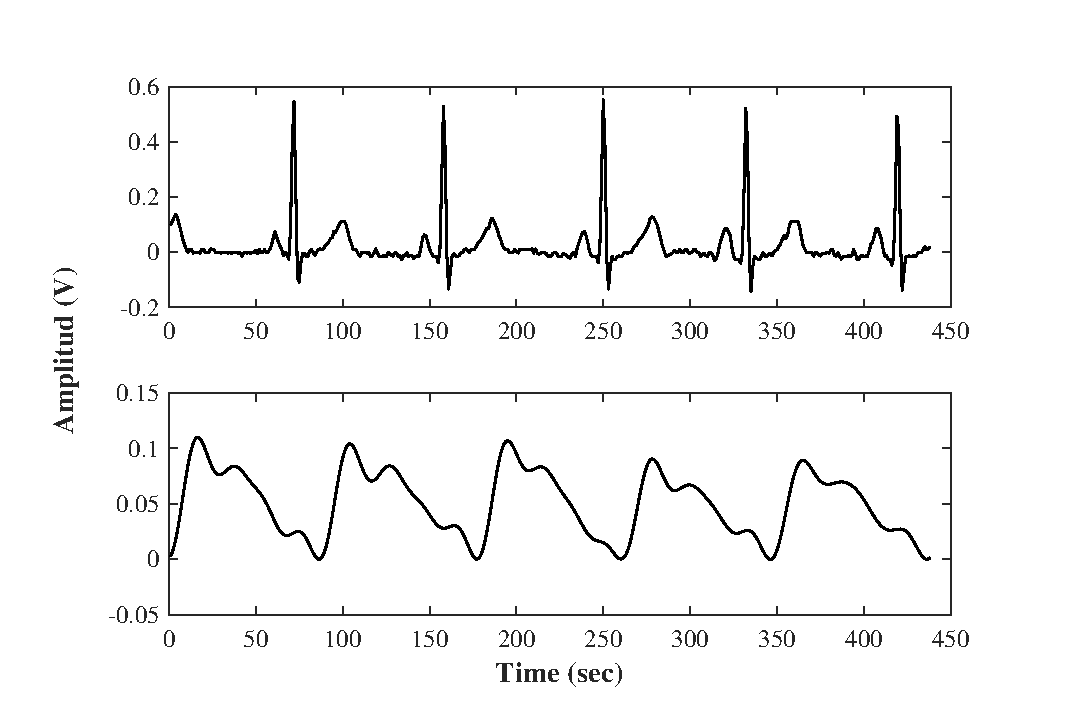
\includegraphics[width=0.75\textwidth,keepaspectratio]{figure3}    
	\caption[Classic plethysmography waveform]{Representation of a classic plethysmography waveform from the heart cycle. The image on the top represents the electrical signal of the heart (ECG). The one below is the plethysmography waveform of the circulation. Both signal are synchronous}
	\label{fig:plethysmography}
\end{figure}

There are different methods and technologies to measure plethysmography. Every method can be applied separately or as part of a system. Some techniques can measure plethysmography of the whole body, segments or localised areas. For instance, chambers of air or water are used to measure lung capacity. This chamber measures the air displacement of a patient while this inhales inside the chamber. 

For measurement of changes of volume of a limb's segment, the air plethysmography technique could be very cumbersome and not very practical. This is one of the many reasons why more techniques have been developed. The following section describes methods to detect plethysmography from a part of the body.

\subsection{Air plethysmography}
\label{section literature 3.1}
Air plethysmography is not a common method to measure a limb’s change of volume. It has been used as an either alternative or research method as explained by Chuah et al.~\cite{chuah2004plethysmography} for measurement of plethysmography without venous occlusion. This approach uses a special chamber that contains the limb in a close area with orifices where transducers and calibration devices are connected. The arm is introduced into the case through a tight rubber sleeve to ensure that the instrument is airtight.  The plethysmography pulsations are detected by measuring the displacement of the surrounding air with a sensor connected to the chamber, which also moves the rubber diaphragm which a Doppler ultrasound transducer measures displacement. As can be noticed, this method could be burdensome, and it is not very desirable to be applied during critical application such as surgery.

\begin{figure}[!htpb]
	\centering
	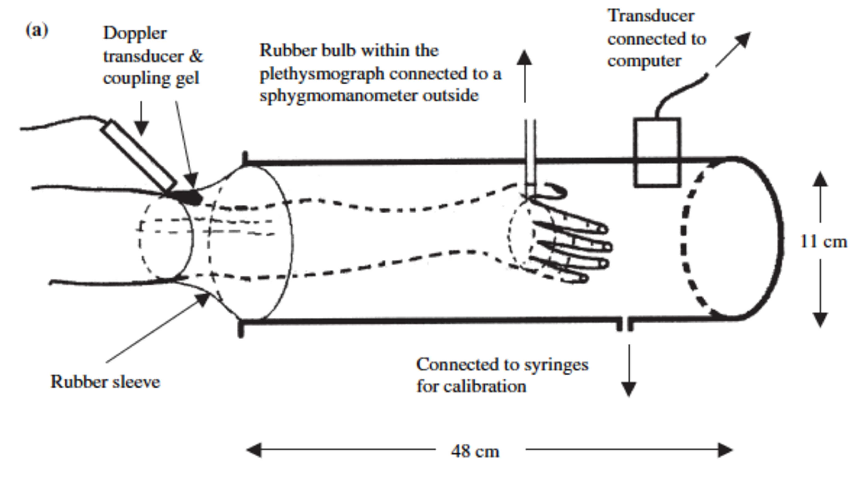
\includegraphics[width=0.95\textwidth,keepaspectratio]{figure4}    
	\caption[Air plethysmography method]{Representation of an air plethysmography device. It requires a one side open cylinder with with a rubber sleeve. There is a compartment where the air displacement caused by each cardiac cycle can be measured.}
	\label{fig:air plethysmography}
\end{figure}

\subsection{Doppler method}
\label{section literature 3.2}
The Doppler technique is not directly a plethysmography method because it does not measure changes in volume but variations of flow. In physics, both parameters are related if the cross-section area of the volume being measured is known. Hence, if the flow and area are known is possible to deduce the volume flow rate. This method uses the Doppler effect to measure blood flow non-invasively from the skin surface. It is very popular in the medical ambit. It could be implemented via ultrasound (ultrasound Doppler flowmetry) frequency or photoelectric effect (laser Doppler flowmetry).  This method measures the velocity of particles in solution using frequency shift of backscattered ultrasound or light~\cite{orekhova2013doppler} (see Figure \ref{fig:Doppler method}). 

A signal is generated to a target tissue and then reflected by the macroscopic tissue structures. Some of the energy in light or sound form is reflected, absorbed and scattered by the tissue and blood particles. This method measures the microcirculation underlying the flow of the arterioles and venules. However, this technique is mainly for superficial measurements or invasively for free flap flow measurements. For instance, it has been studied that laser Doppler flowmetry has \SI{1}{\milli\meter} of penetration. In the case of ultrasound Doppler measurements are affected by the angle of the frequency applied to the target tissue.

\mynote{reference to this depth}

\begin{figure}[!htpb]
	\centering
	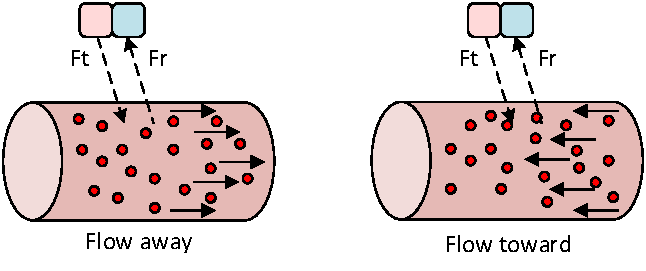
\includegraphics[width=0.75\textwidth,keepaspectratio]{figure5}    
	\caption[Doppler technique to measure flow]{Representation of a classic plethysmography waveform from the heart cycle. The image on the top represents the electrical signal of the heart. The one before is the plethysmography waveform of the circulation.}
	\label{fig:Doppler method}
\end{figure}


\subsection{Strain gauge plethysmography}
\label{section literature 3.3}
This method also known as SGP (strain gauge plethysmography) is a non-invasive method to quantify retrograde outflow in the deep venous system and peripheral arterial disease~\cite{holohan1996plethysmography}. It works by applying a strain gauge around the limb under test. The transducer could be a tube filled in with a conductive material such as mercury and gallium and connected to a source of electricity. However, alternative methods that do not use clinically banned mercury have been developed using electrical conductive fluids~\cite{flowers1981strain}. When the gauge experiences variations of circumference caused by a change of volume of the rib cage or the pulse in a limb, the resistance of the sensor also vary accordingly obtaining an electrical waveform. To increase sensitivity for venous filling measurements occlusion cuffs would be required, as shown in Figure~\ref{fig:strain gauge}. This method does not provide reliable quantitative data for venous occlusion but provides qualitative data for the function of the extremity in venous insufficiency~\cite{holohan1996plethysmography}. 

\begin{figure}[!htpb]
	\centering
	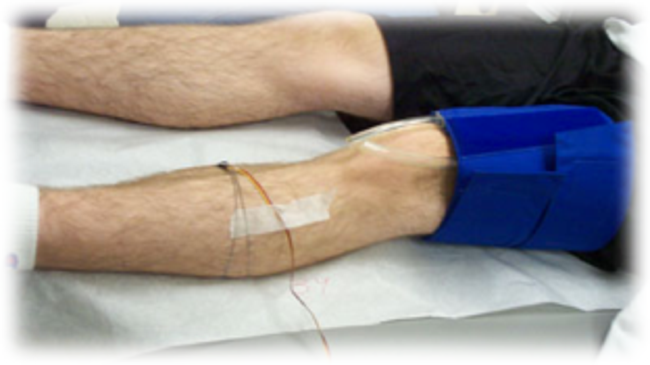
\includegraphics[width=0.75\textwidth,keepaspectratio,trim={0.5cm 0.5cm 0.5cm 0.5cm}, clip]{figure6}    
	\caption[Strain gauge plethysmography]{Representation of a classic plethysmography waveform from the heart cycle. The image on the top represents the electrical signal of the heart. The one before is the plethysmography waveform of the circulation.}
	\label{fig:strain gauge}
\end{figure}


\subsection{Photoelectric method}
\label{section literature 3.4}
This method is technically known as photoelectric plethysmography or PPG for short. It is one of the most popular methods used in medical applications nowadays. It is a non-invasive method that uses different light wavelengths to obtain a plethysmography graph. It is widely used for monitoring or evaluating heart rate, oxygen saturation, peripheral arterial pressure and peripheral microcirculation after skin grafting, drug ingestion, burns or revascularization~\cite{holohan1996plethysmography}. There are two different techniques to obtain readings. One is transmission-mode (see figure \ref{fig:PPG transmission}.) that works by placing the tissue of interest (i.e. finger, toe or ear lobe) between the light emitting diode (LED) and the photoreceptor (PD).  The other is PPG reflectance-mode (see figure\ref{fig:PPG reflectance}) by placing the LED next to photoelectric cell over the surface of the tissue o study. PPG uses the AC component of the signal for arterial pulse detection and the DC component for venous evaluation~\cite{higgins1986photoplethysmographic}. It also uses a different kind of wavelengths to avoid interference from external sources of light. The principle behind PPG is the detection of the degree of attenuation of backscatter light from the superficial layers of skin about \SIrange{1.5}{2.0}{\milli\meter} ~\cite{holohan1996plethysmography,kim1986pulse}. The amount of reflected light varies with the total number of RBC’s in the cutaneous microcirculation, which alters the wavelength during each cardiac cycle. This method has been proved to be effective for the initial diagnostics of peripheral arterial disease (PAD) and chronic peripheral venous insufficiency (CVI).

Some of the disadvantages of PPG are that only measures a small area at the time. Therefore, it is not possible to get a spatial distribution of the blood volume change over the skin~\cite{wu2003ppgi}. Also, skin pigmentation has been probed being an error factor as well as nail polishers~\cite{fallow2013influence}. 

\begin{figure*}[!htbp]
	\centering
	\begin{subfigure}[t]{0.45\textwidth}
		\centering
		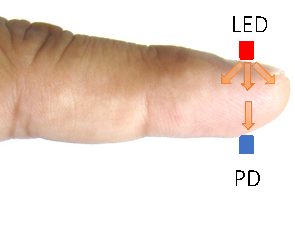
\includegraphics[height=4cm]{figure7a}
		\caption{Placement of LED and photodetector in transmission mode}
		\label{fig:PPG transmission}
	\end{subfigure}%
	~ 
	\begin{subfigure}[t]{0.45\textwidth}
		\centering
		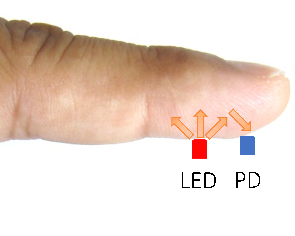
\includegraphics[height=4cm]{figure7b}
		\caption{Placement of LED and photodetector in reflectance mode}
		\label{fig:PPG reflectance}
	\end{subfigure}
	\caption[PPG sensors placemens as transmission and reflectance modes]{PPG light emitter placement and receptor according to the mode, transmission and reflectance}
	\label{fig:PPG modes}
\end{figure*}

\subsection{Bioelectrical Impedance}
\label{section literature 3.5}
Also known as impedance plethysmography (iPG) involves the measurement of the change in impedance due to change of blood flow. For instance, when heart’s systole increases blood flow, the volume of a limb rises due to the inflow of blood (swelling)~\cite{martinsen2011bioimpedance}. Consequently, there are changes of impedance correlated to the changes of volume and flow in a limb. Some medical application might require the use of occlusion cuffs to analyse venous filling. There are several medical applications for this kind of technique such as heart stroke volume (SV) measurement, cardiac output (CO), thoracic respiratory volume, oedema and detection of deep vein thrombosis (DVT)~\cite{holohan1996plethysmography}.

The following section describes more in detail the definition of iPG, how it works, medical applications, how is measured and the possible ways to represent it. This information will help to understand how volume and ischemia can be related to calculating an index between the two measurements.

%********************************** %Nomenclatures in chapter  **************************************
\nomenclature[z-Hb]{Hb}{Haemoglobin}
\nomenclature[z-ATP]{ATP}{Adenosine Triphosphate}
\nomenclature[z-rbc]{RBC}{Red Blood Cells}
\nomenclature[z-abi]{ABI}{Ankle-Branchial index}
\nomenclature[z-wbc]{WBC}{White Blood Cells}
\nomenclature[z-PVD]{PVD}{Peripheral vascular disease}
\nomenclature[z-bia]{BIA}{Bioelectrical impedance analysis}
\nomenclature[z-DFI]{DFI}{Doppler flowmetry}
\nomenclature[z-DVT]{DVT}{Deep vein thrombosis}
\nomenclature[z-cli]{CLI}{Critical Limb Ischemia}
\nomenclature[z-PAD]{PAD}{Peripheral Arterial Disease}
\nomenclature[z-SV]{SV}{Strove Volume}
\nomenclature[z-LED]{LED}{Light emitting diode}
\nomenclature[z-CVI]{CVI}{Chronic peripheral venous insufficiency}
\nomenclature[z-ppg]{PPG}{Photoplethysmography}
\nomenclature[z-ipg]{iPG}{Impedance Plethysmography}
\nomenclature[z-CO]{CO}{Cardiac output}
\nomenclature[z-SGP]{SGP}{strain gauge plethysmography}
\nomenclature[z-BIA]{BIA}{Bioelectrical impedance analysis}


%\nomenclature[z-cif]{$CIF$}{Cauchy's Integral Formula}                                % first letter Z is for Acronyms 
%\nomenclature[a-F]{$F$}{complex function}                                                   % first letter A is for Roman symbols
%\nomenclature[g-p]{$\pi$}{ $\simeq 3.14\ldots$}                                             % first letter G is for Greek Symbols
%\nomenclature[g-i]{$\iota$}{unit imaginary number $\sqrt{-1}$}                      % first letter G is for Greek Symbols
%\nomenclature[g-g]{$\gamma$}{a simply closed curve on a complex plane}  % first letter G is for Greek Symbols
%\nomenclature[x-i]{$\oint_\gamma$}{integration around a curve $\gamma$} % first letter X is for Other Symbols
%\nomenclature[r-j]{$j$}{superscript index}                                                       % first letter R is for superscripts
%\nomenclature[s-0]{$0$}{subscript index}                                                        % first letter S is for subscriptsd
